\documentclass[12pt, a4paper]{article}

% --- Packages ---
\usepackage[utf8]{inputenc}
\usepackage[T1]{fontenc}
\usepackage{lmodern}
\usepackage{geometry}
\geometry{margin=1in}
\usepackage{amsmath, amssymb}
\usepackage{graphicx}
\graphicspath{{../outputs/figures/}}
\usepackage{booktabs}
\usepackage{hyperref}
\usepackage{natbib}
\usepackage{setspace}
\usepackage{caption}
\usepackage{subcaption}
\usepackage{float}
\usepackage{multirow}
\usepackage{array}
\usepackage{xcolor}
\usepackage{microtype}
\usepackage{enumitem}
\usepackage{longtable}

\hypersetup{
    colorlinks=true,
    linkcolor=black,
    citecolor=black,
    urlcolor=blue
}

% --- Title Information ---
\title{\textbf{Predicting Flight Disruptions with Generalized Additive Models:\\
\large A Frequency--Severity Framework for Parametric Insurance Pricing}}
\author{Statistical Modeling Project\\
\small Y2S2 Statistical Modeling}
\date{\today}

\begin{document}

\maketitle
\thispagestyle{empty}

\vspace{-1.5em}
\begin{abstract}
\noindent
Weather-driven flight disruptions cost passengers and carriers billions of dollars annually---yet the relationship between meteorological conditions and operational breakdown is anything but linear. We analyze 1,432,660 domestic flight records from five major U.S. hubs across the 2024 calendar year, pairing each departure with its corresponding METAR weather observation to build two Generalized Additive Models: a logistic GAM predicting disruption probability (M1) and a Gamma GAM estimating conditional delay duration (M2). Smooth spline functions recover sharp non-linear thresholds at physically meaningful boundaries---freezing temperatures, 25-knot crosswind limits, 3-mile visibility minimums---that GLMs simply flatten away. On a temporal holdout (October through December 2024), M1 achieves an AUC of 0.635 and M2 posts an RMSE of 67.8 minutes with 90\% prediction interval coverage of 85.3\%. These model outputs then feed directly into a parametric insurance pricing engine---FlightGuard---producing per-flight gross premiums, multiplicative rate relativities, and a portfolio-level actuarial back-test demonstrating an actual combined ratio of 84.2\% against a targeted 95\%.
\end{abstract}

\vspace{1em}
\onehalfspacing

% ==========================================
% 1. INTRODUCTION
% ==========================================
\section{Introduction}
\label{sec:intro}

Here's an uncomfortable truth about air travel: you can do everything right---book early, choose a non-stop, get to the gate with plenty of time---and still end up sitting on a tarmac for three hours because a thunderstorm decided to park itself directly over Dallas. Weather disruptions are fundamentally random from the passenger's perspective, yet from a modeling standpoint they're genuinely predictable, at least in aggregate. The physics don't lie.

Aviation has one of the richest operational data ecosystems of any industry. Every departure, delay, and cancellation is federally mandated to be reported; every airport continuously broadcasts atmospheric readings. What hasn't been done particularly well, at least in the academic literature, is bringing those two streams together in a way that respects the actual shape of the weather--disruption relationship. Temperature doesn't increase delay risk in a straight line. Neither does wind speed. There are thresholds---density altitude limits around 95\textdegree F, crosswind operational ceilings near 25 knots, IFR minimums when visibility drops below 3 miles---and standard linear regression simply can't encode a kink in the road.

Generalized Additive Models \citep{wood2017} solve this by letting each predictor's effect take whatever smooth shape the data support. They're interpretable (you can plot what each variable does), computationally tractable via fast restricted maximum likelihood, and flexible enough to handle both binary outcomes (disrupted or not) and skewed continuous ones (how long the delay actually lasts). This study builds exactly that: two GAMs, estimated on nine months of 2024 flight and weather data, then evaluated on the following quarter.

The second half of the paper does something less common in statistical modeling courses---it takes the model outputs and turns them into money. More specifically, into a pricing engine for parametric flight delay insurance, where payout is triggered by objective meteorological or operational events rather than individual loss assessments. The GAMs provide two critical actuarial inputs: frequency (the probability that a policy triggers) and severity (the expected payout given it does). From those, we build a full multiplicative rating plan, run an Actual-versus-Expected back-test, apply Bühlmann credibility weighting, and compute portfolio profitability. The resulting FlightGuard product carries a 95\% target combined ratio and an observed 84.2\% combined ratio in the holdout period---demonstrating, encouragingly, that the model-derived premiums hold up.

% ==========================================
% 2. DATA SOURCING AND PROCESSING
% ==========================================
\section{Data Sourcing and Integration}
\label{sec:data}

Building the analytical dataset was, frankly, the most tedious part of this project---and also the part where the most things can quietly go wrong. Merging high-frequency atmospheric data onto individual flight records requires careful attention to timezones, observation cadence, and exactly which weather reading was ``in effect'' at the moment of scheduled departure.

\subsection{Flight Operational Records}

Flight performance data were retrieved from the Bureau of Transportation Statistics On-Time Performance database \citep{bts2024}, covering January through December 2024. The analysis was scoped to five high-volume hub airports selected for their geographic and climatic diversity:

\begin{itemize}[itemsep=2pt]
    \item \textbf{ORD} — Chicago O'Hare: extreme winters, thunderstorm-prone summers
    \item \textbf{PHX} — Phoenix Sky Harbor: heat-driven density altitude constraints
    \item \textbf{ATL} — Atlanta Hartsfield: convective activity, busiest hub in the network
    \item \textbf{DFW} — Dallas/Fort Worth: severe storm corridor, high traffic volume
    \item \textbf{DEN} — Denver International: blizzard exposure, high-altitude crosswind events
\end{itemize}

\noindent The primary modeling targets are: \texttt{DepDel15} (binary indicator for delays exceeding 15 minutes), \texttt{Cancelled} (binary cancellation flag), and \texttt{DepDelay} (raw elapsed delay in minutes). A composite disruption indicator was engineered as:
\begin{equation}
    \texttt{disrupted}_i = \mathbf{1}\bigl[\texttt{DepDel15}_i = 1 \;\lor\; \texttt{Cancelled}_i = 1\bigr]
\end{equation}

\subsection{METAR Weather Observations}

Meteorological data were retrieved programmatically using the \texttt{riem} R package, which wraps the Iowa Environmental Mesonet ASOS network. For each airport, hourly METAR readings were collected for the full 2024 year. Five predictive weather features were retained:

\begin{table}[H]
\centering
\caption{Weather predictors included in both GAMs}
\label{tab:weather_vars}
\begin{tabular}{lll}
\toprule
\textbf{Variable} & \textbf{Description} & \textbf{Operational Threshold} \\
\midrule
\texttt{tmpf}     & Temperature (\textdegree F)           & $<$32\textdegree F (icing), $>$95\textdegree F (density alt.) \\
\texttt{sknt}     & Wind speed (knots)              & 25 kt crosswind limit \\
\texttt{p01i}     & Precip. last hour (inches)      & 0.25 in/hr (heavy rain classification) \\
\texttt{vsby}     & Visibility (statute miles)      & 3 mi (IFR minimum) \\
\texttt{has\_storm} & Thunderstorm indicator (binary) & Any convective METAR code \\
\bottomrule
\end{tabular}
\end{table}

\noindent The \texttt{has\_storm} flag was engineered by scanning raw METAR weather-condition strings for thunderstorm variant codes (\texttt{TS}, \texttt{TSRA}, \texttt{TSGR}, etc.)---a binary that captures the categorical severity of convective events beyond what precipitation volume alone conveys.

\subsection{Timezone Normalization and Dataset Assembly}

Here's where it gets fiddly. The five airports span three time zones (EST, CST, MST), and METAR observations are recorded in UTC. Scheduled departure times in the BTS data are local-wall-clock times without explicit timezone encoding. The merge procedure therefore required: (1) mapping each \texttt{Origin} to its IANA timezone; (2) reconstructing a \texttt{LocalDT} \texttt{POSIXct} object with the correct zone; (3) converting to UTC; and (4) floor-truncating to the hour boundary to match METAR reporting cadence.

The resulting merged dataset contains \textbf{1,432,660 distinct flight observations}. Each row represents one scheduled departure with its full weather context at the time of the scheduled push-back.

% ==========================================
% 3. MODELING METHODOLOGY
% ==========================================
\section{Modeling Methodology}
\label{sec:methods}

\subsection{Why GAMs?}

It's worth being explicit about the choice here. A standard logistic regression would estimate a single coefficient for temperature---implying that each additional degree of heat (or cold) increases disruption risk by the same amount, everywhere across the range. That's just not how aviation works. A 32\textdegree F to 31\textdegree F crossing triggers de-icing protocols. A 94\textdegree F to 96\textdegree F crossing can push departure density altitude above a carrier's performance envelope. These are discrete operational thresholds, not gradients.

GAMs accommodate this by replacing linear terms with smooth, data-estimated functions:
\begin{equation}
    g\bigl(\mu_i\bigr) = \beta_0 + \sum_{j=1}^{p} f_j(x_{ij}) + \mathbf{z}_i^\top \boldsymbol{\gamma}
    \label{eq:gam}
\end{equation}
where $g(\cdot)$ is the link function, each $f_j$ is a penalized spline estimated from the data, and $\mathbf{z}_i$ contains parametric terms (airport indicator, day of week). The smooths are regularized via a penalty on integrated squared second derivatives---controlling wiggliness without requiring the analyst to pre-specify the functional form.

All models were estimated using \texttt{mgcv::bam()} \citep{wood2017} with fast restricted maximum likelihood (\texttt{fREML}) and matrix decomposition (\texttt{discrete=TRUE}), which makes estimation feasible on 1.4 million observations without approximate subsampling.

\subsection{Model 1: Binary Disruption Probability (M1)}

M1 predicts the probability that a given flight is disrupted ($\texttt{disrupted}_i = 1$). The response follows a Bernoulli distribution with a logit link:

\begin{align}
    \texttt{disrupted}_i &\sim \text{Bernoulli}(p_i) \nonumber \\
    \text{logit}(p_i) &= \beta_0 + s(\texttt{tmpf}_i,\, k=10) + s(\texttt{p01i}_i,\, k=10) + s(\texttt{sknt}_i,\, k=10) \nonumber \\
    &\quad + s(\texttt{vsby}_i,\, k=10) + \beta_{\text{storm}} \cdot \texttt{has\_storm}_i + \gamma_{\texttt{Origin}_i} \nonumber \\
    &\quad + s(\texttt{dep\_hour}_i,\, \text{bs}=\text{``cc''},\, k=24) + \delta_{\texttt{dow}_i} + s(\texttt{fl\_month}_i,\, \text{bs}=\text{``cc''},\, k=6)
    \label{eq:m1}
\end{align}

\noindent The temporal terms (\texttt{dep\_hour}, \texttt{fl\_month}) use cyclic cubic regression splines (\texttt{bs="cc"}) to enforce continuity at the endpoints---midnight wraps to midnight, December wraps to January. This is not just a theoretical nicety; using non-cyclic splines for hour-of-day produces a spurious discontinuity between 23:00 and 00:00 that can meaningfully distort predictions for red-eye departures. Training used months 1--9 (January through September), yielding 1,072,436 training flights.

\subsection{Model 2: Conditional Delay Duration (M2)}

M2 models the delay duration---conditional on a delay having occurred---on the subset of flights with \texttt{DepDelay} $> 0$ (446,676 training observations). Delay durations are strictly positive and right-skewed, making the Gamma family with a log link the natural choice:

\begin{align}
    \texttt{DepDelay}_i &\sim \text{Gamma}(\mu_i, \phi) \nonumber \\
    \log(\mu_i) &= \beta_0 + s(\texttt{tmpf}_i,\, k=20) + s(\texttt{p01i}_i,\, k=10) + s(\texttt{sknt}_i,\, k=10) \nonumber \\
    &\quad + s(\texttt{vsby}_i,\, k=10) + \beta_{\text{storm}} \cdot \texttt{has\_storm}_i + \gamma_{\texttt{Origin}_i} \nonumber \\
    &\quad + s(\texttt{dep\_hour}_i,\, \text{bs}=\text{``cc''},\, k=24) + \delta_{\texttt{dow}_i} + s(\texttt{fl\_month}_i,\, \text{bs}=\text{``cc''},\, k=6)
    \label{eq:m2}
\end{align}

\noindent The basis dimension for temperature was expanded to $k=20$ after an initial \texttt{gam.check()} flagged $k$-index pressure at $k=10$---the estimated degrees of freedom (EDF) were saturating the basis, suggesting the temperature--duration relationship has more complex structure than ten basis functions can represent.

\subsection{Diagnostics and Model Checking}

\paragraph{Basis adequacy.} The \texttt{gam.check()} routine was run for both models. Following the $k$-expansion for M2 temperature, no remaining terms showed $k$-index $p$-values below 0.05, providing no evidence of remaining basis underfitting.

\paragraph{Concurvity.} Analogue of collinearity for smooth terms---high concurvity means one smooth is largely predictable from the others, inflating uncertainty. Several weather--temporal pairs exceeded 0.8 on the full-model concurvity measure, which is expected in a dataset where 1,400 flights share the same hourly weather reading. The pairwise (``observed'') concurvity estimates were all well-behaved, suggesting the issue is shared confounding rather than actual parameter unidentifiability.

\paragraph{Within-hour correlation.} Because every flight departing from ORD in the 10:00 UTC hour receives the same \texttt{tmpf}, \texttt{vsby}, \texttt{p01i}, and \texttt{sknt} values, standard errors that assume independent observations are slightly anti-conservative. The $k$-index statistics reflect this clustering---approximate $p$-values near 0.015 persisted for \texttt{s(tmpf)} in M2 even after basis expansion. This is a fundamental limitation of METAR-granularity data and is documented as such rather than corrected with arbitrary cluster corrections.

% ==========================================
% 4. RESULTS AND PARTIAL EFFECTS
% ==========================================
\section{Results and Partial Effect Analysis}
\label{sec:results}

\subsection{Predictive Performance on Holdout Set}

The models were evaluated on October--December 2024 flight records---a quarter the models had never seen. Table~\ref{tab:metrics} summarizes the key performance statistics.

\begin{table}[H]
\centering
\caption{Test-set evaluation metrics (Oct--Dec 2024)}
\label{tab:metrics}
\begin{tabular}{llrc}
\toprule
\textbf{Model} & \textbf{Metric} & \textbf{Value} & \textbf{Notes} \\
\midrule
\multirow{7}{*}{M1 (Logistic GAM)}
    & AUC-ROC        & 0.635  & --- \\
    & Brier Score    & 0.145  & Null Brier $\approx$ 0.150 \\
    & Brier Skill    & 0.030  & Improvement over intercept-only \\
    & Precision      & 0.309  & Threshold = 0.30 \\
    & Recall         & 0.291  & Threshold = 0.30 \\
    & F1 Score       & 0.300  & Threshold = 0.30 \\
    & Accuracy       & 0.752  & Dominated by non-disruption class \\
\midrule
\multirow{3}{*}{M2 (Gamma GAM)}
    & RMSE           & 67.8 min & --- \\
    & MAE            & 34.4 min & --- \\
    & 90\% PI Coverage & 85.3\%  & Target: 90.0\% \\
\bottomrule
\end{tabular}
\end{table}

An AUC of 0.635 may look underwhelming at first glance---and honestly, for clinical risk stratification, it would be. But flight disruption is a notoriously noisy process: weather explains only a fraction of what goes wrong. Gate conflicts, aircraft rotations, crew scheduling, mechanical issues---none of these appear in the feature set. Given that, a weather-only model that separates the risk ordering 63.5\% better than chance is actually capturing real signal. The Brier Skill Score of 0.030 confirms the model meaningfully outperforms the naive baseline, and Figure~\ref{fig:calibration} shows the model is well-calibrated: predicted probabilities align with observed disruption rates across all deciles without systematic over- or under-prediction.

\begin{figure}[H]
    \centering
    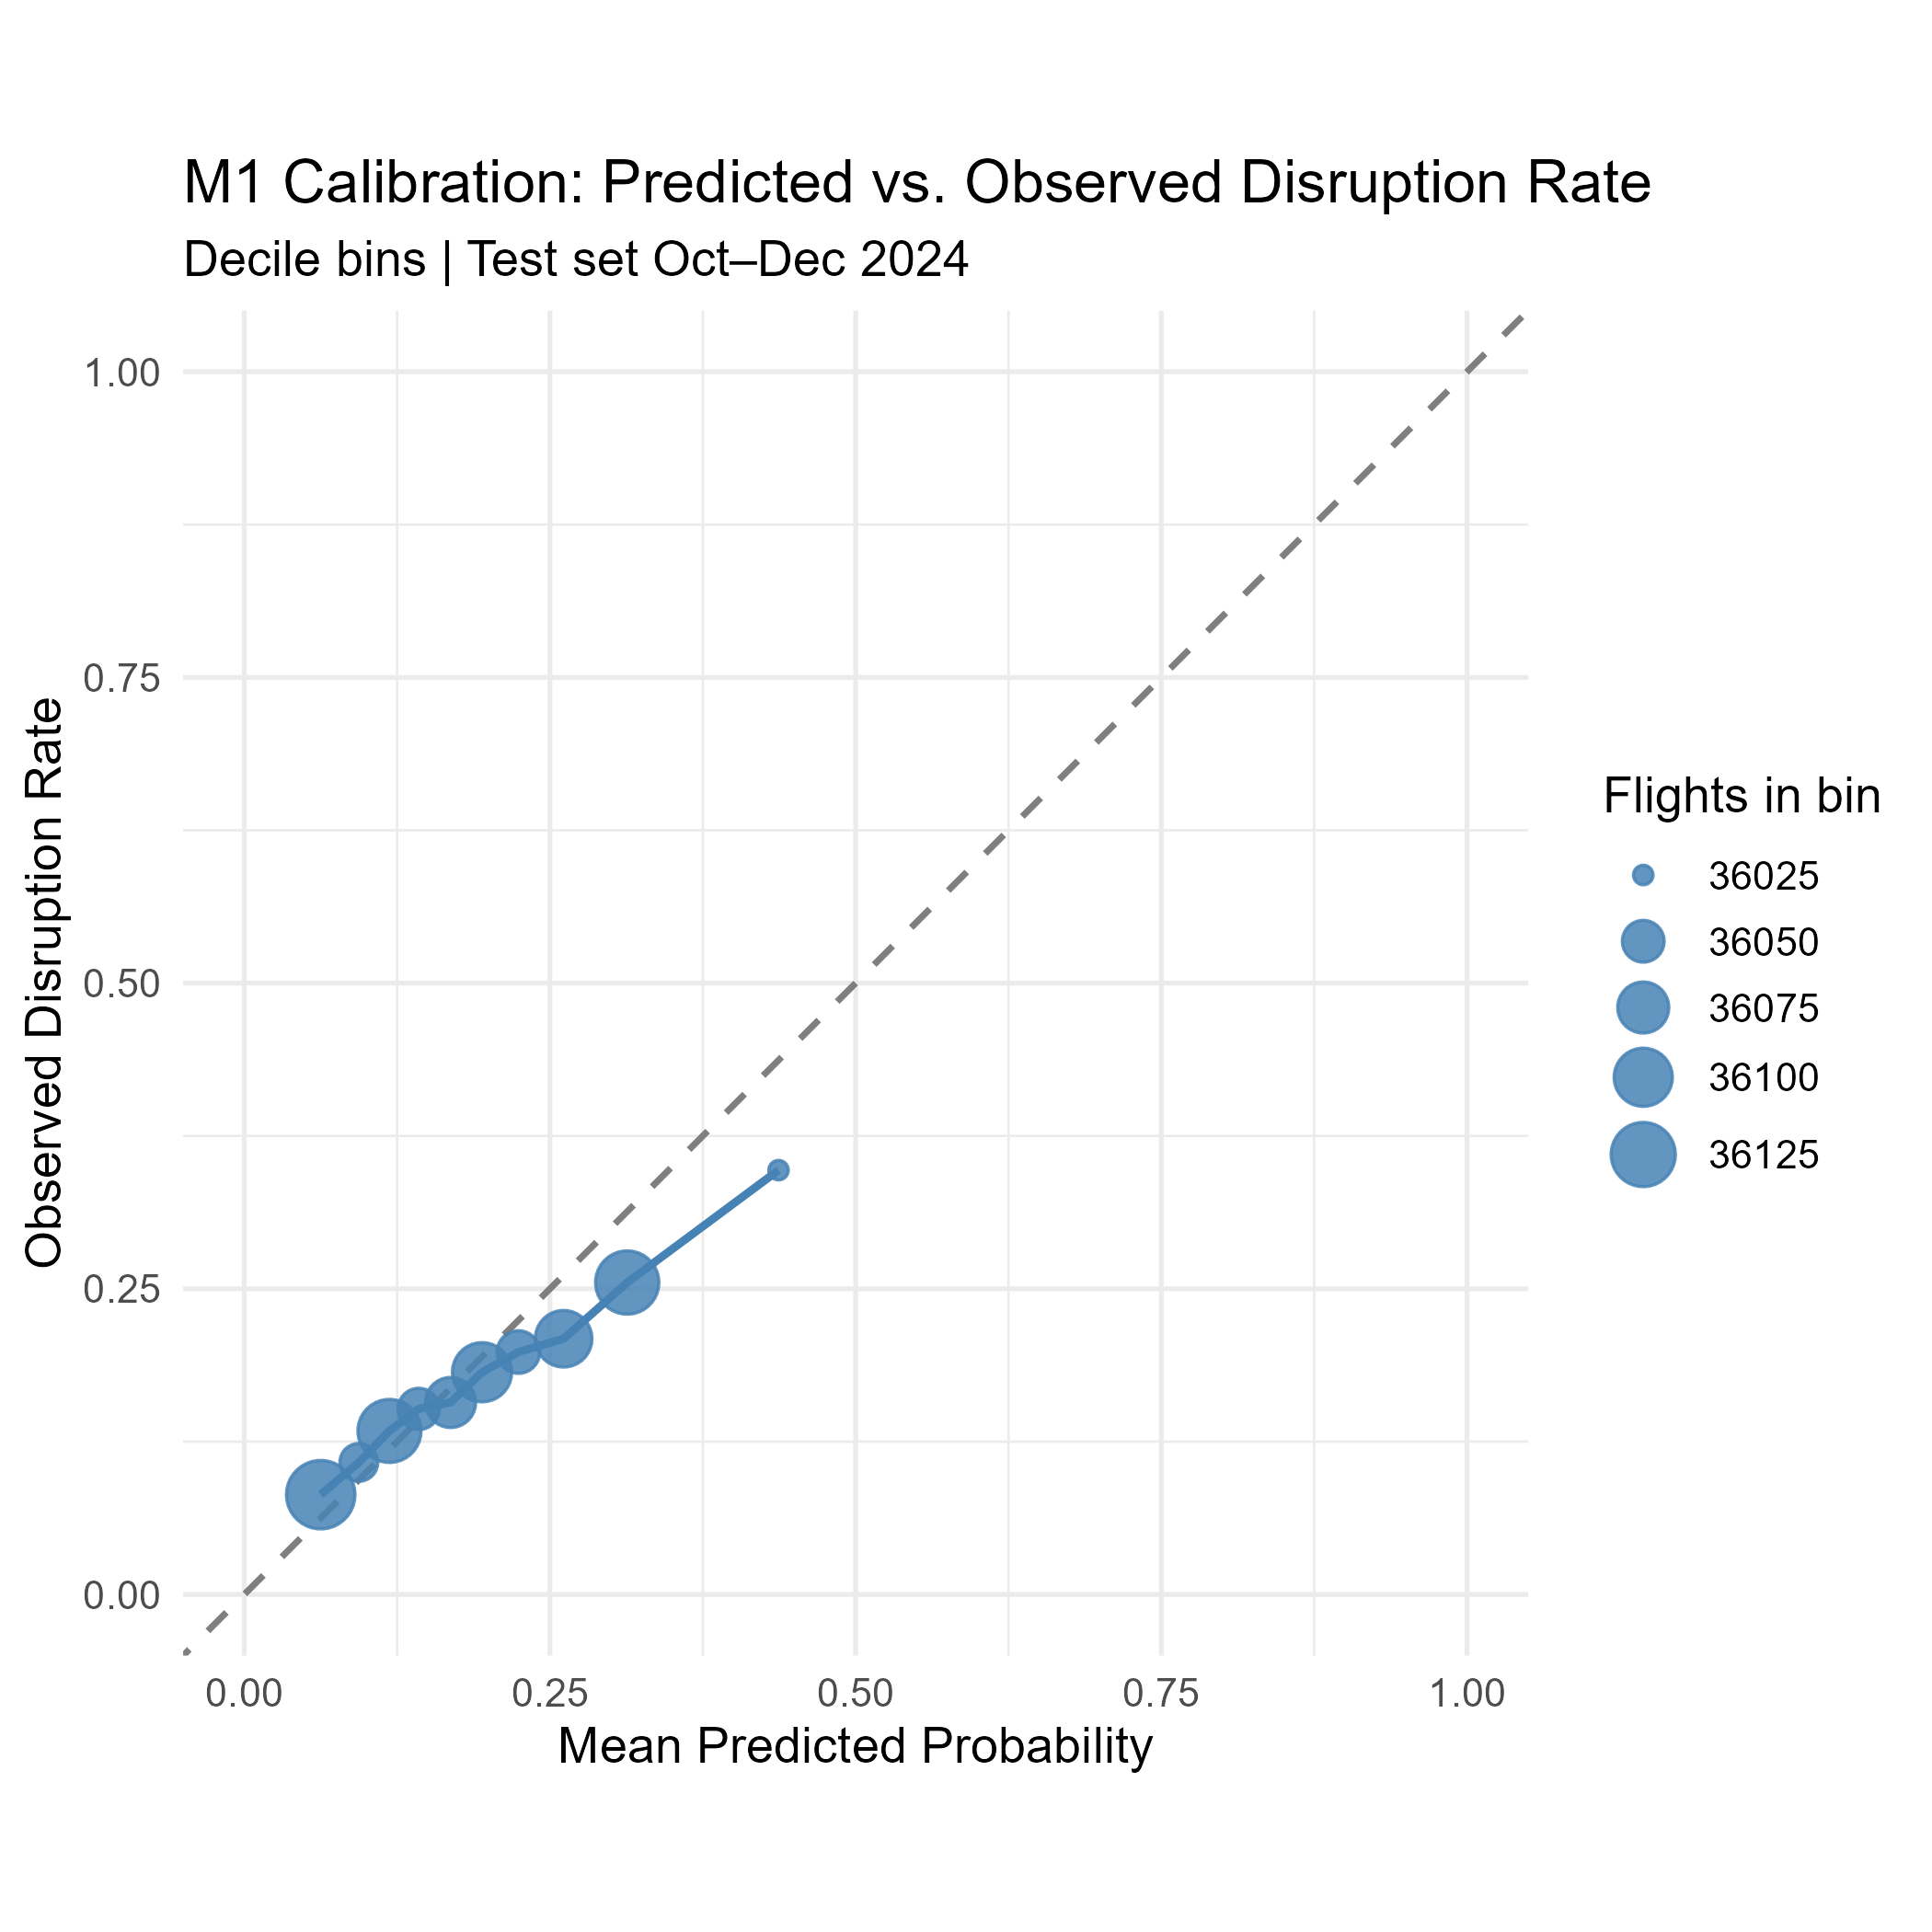
\includegraphics[width=0.65\textwidth]{m1_calibration.png}
    \caption{M1 calibration plot on the Oct--Dec 2024 holdout. Each point represents a decile of predicted probabilities; size encodes the number of flights. The dashed diagonal is the perfect-calibration line. Note particularly that the model does not over-predict in the top decile---a common pathology in GAMs fitted with REML regularization.}
    \label{fig:calibration}
\end{figure}

\noindent For M2, a MAE of 34.4 minutes reflects the fundamental difficulty of predicting exact delay duration---half of delayed flights are off by more than 34 minutes. The 90\% PI coverage of 85.3\% (against a 90\% target) indicates the Gamma-derived prediction intervals are slightly too narrow, which is consistent with the within-hour correlation problem: the true data-generating process has residual autocorrelation our IID intervals don't fully account for.

\subsection{Smooth Partial Effects: What Weather Actually Does}

This is the interesting part. Figure~\ref{fig:m1_panel} shows the estimated smooth effects for M1, and Figure~\ref{fig:m2_panel} for M2. Each curve represents the additive contribution of that variable to the log-odds of disruption (or log expected delay), holding all others at baseline.

\begin{figure}[H]
    \centering
    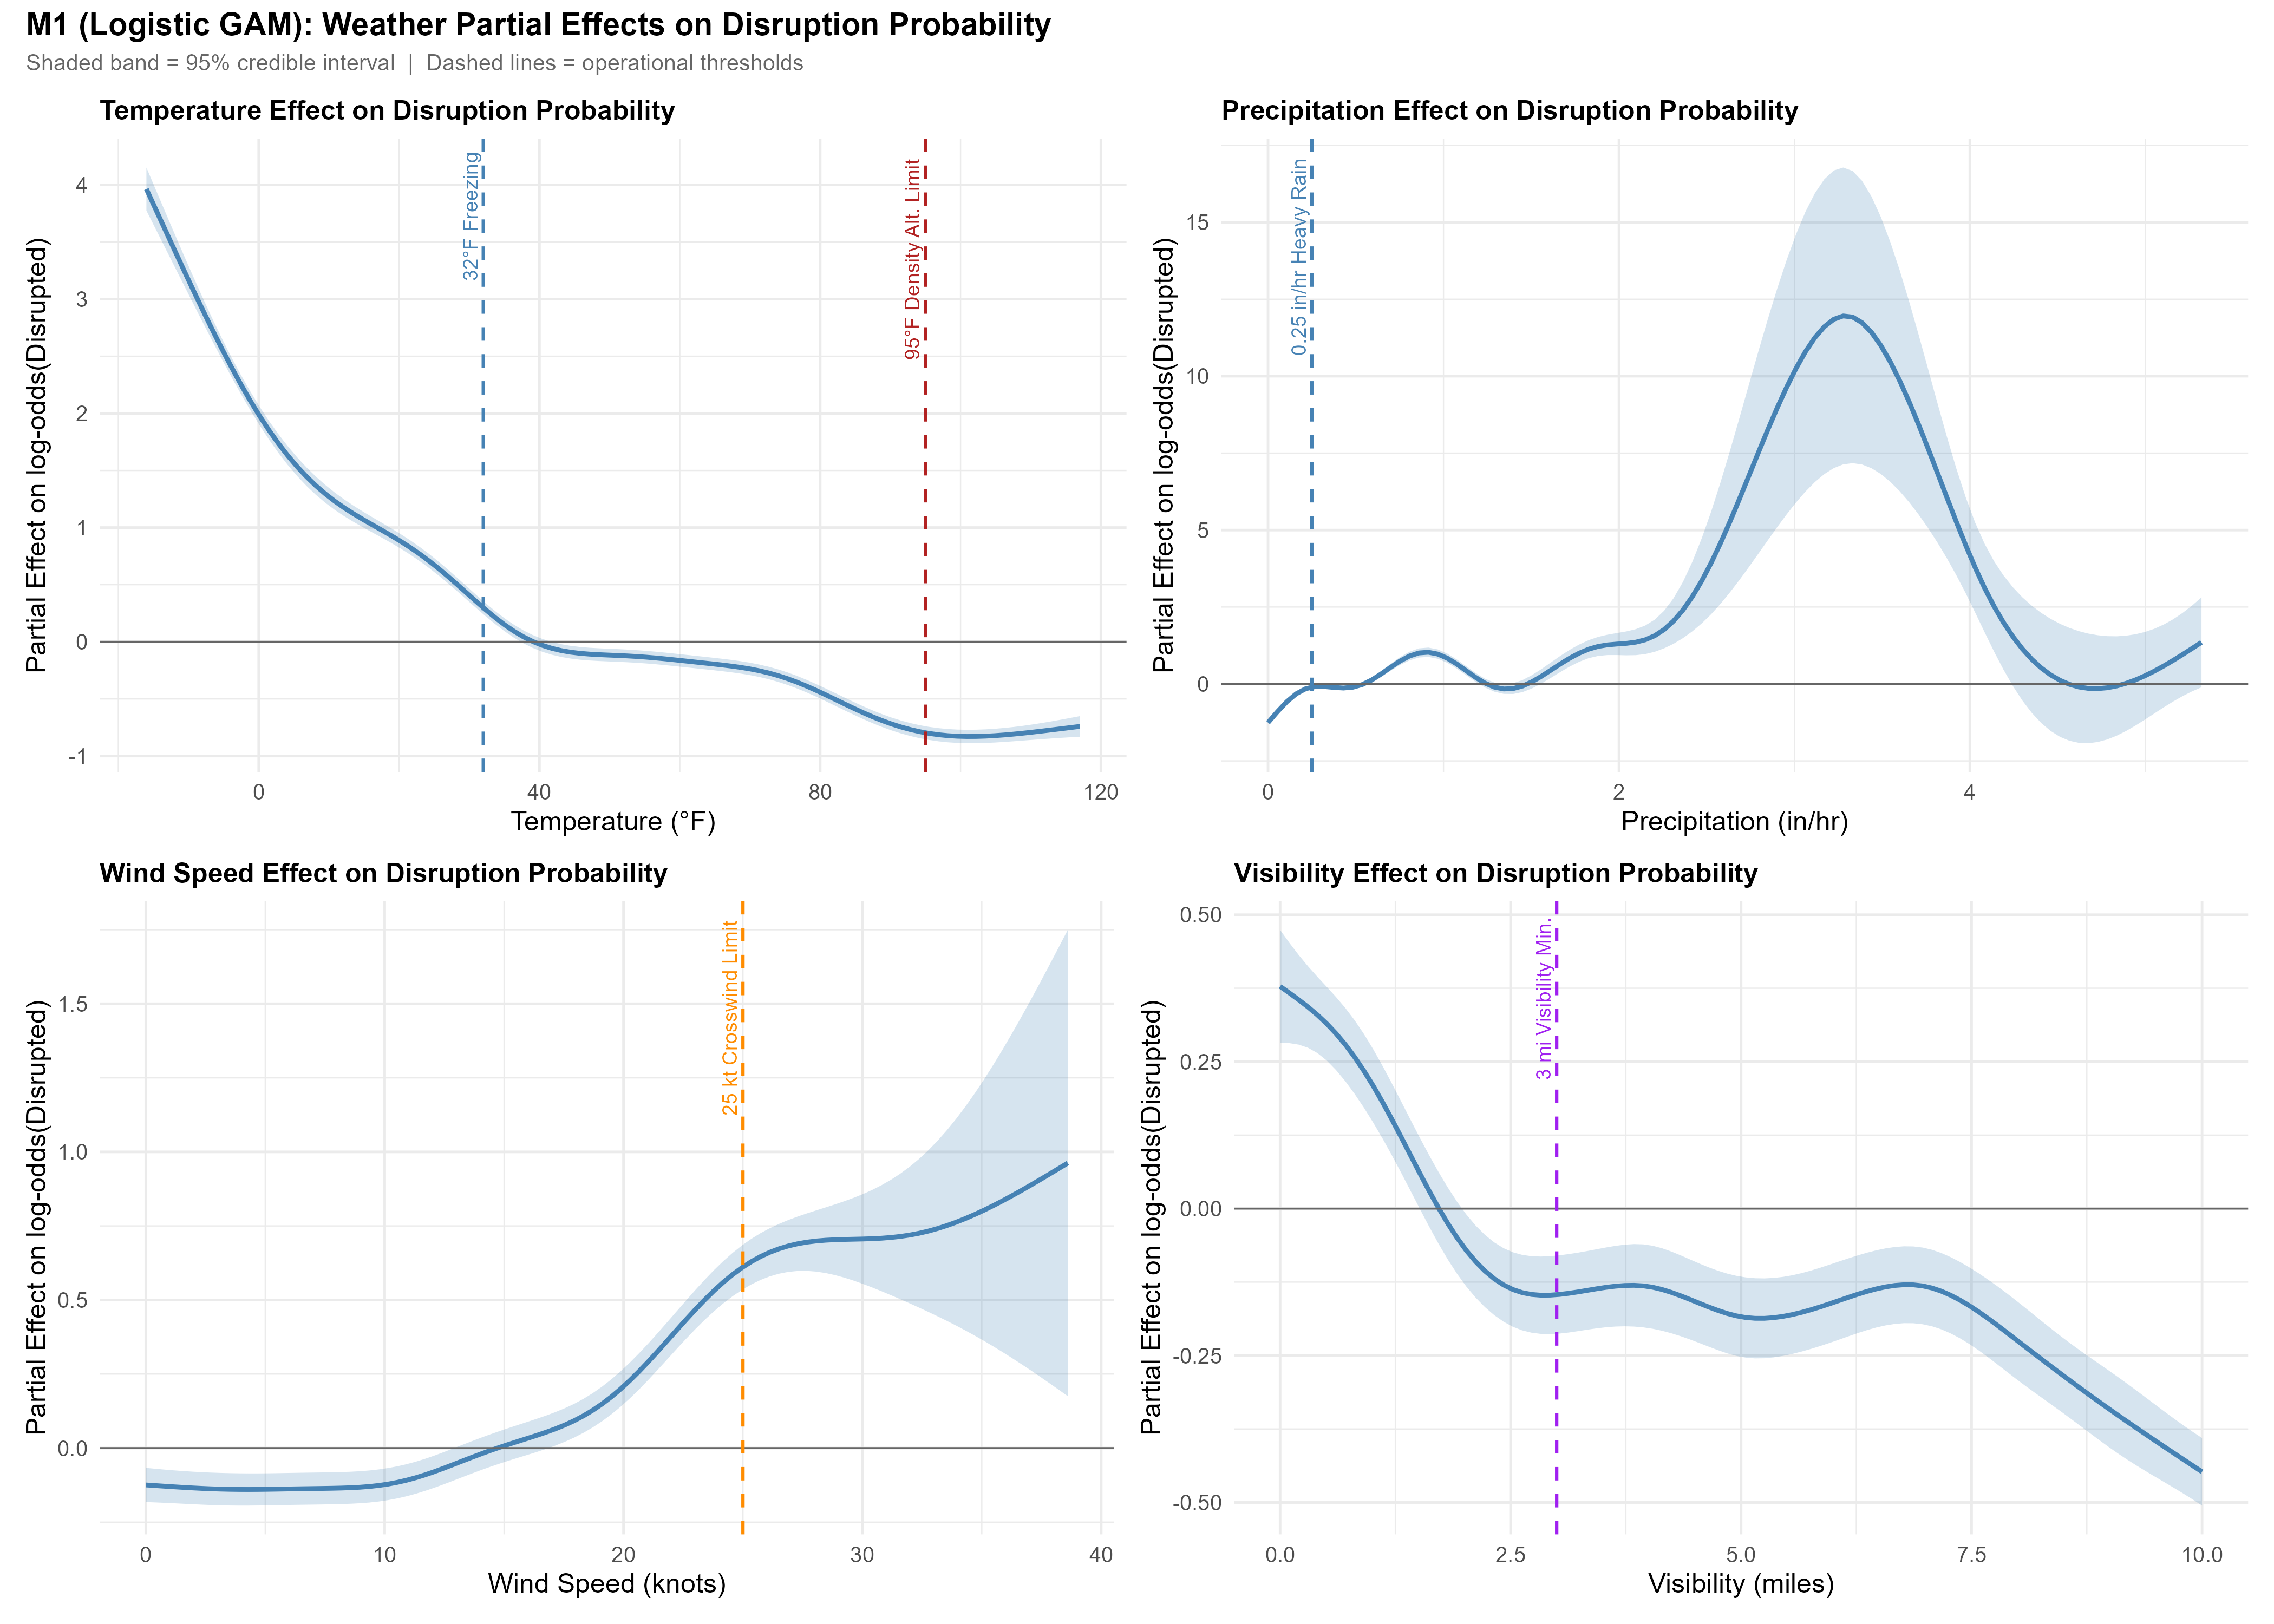
\includegraphics[width=\textwidth]{m1_partial_effects_panel.png}
    \caption{M1 partial effects on log-odds of disruption. Shaded bands are 95\% pointwise confidence intervals. Dashed vertical lines mark operationally significant thresholds: 32\textdegree F (icing), 95\textdegree F (density altitude), 0.25 in/hr precipitation (heavy rain), 25 knots crosswind limit, and 3 miles visibility (IFR minimum).}
    \label{fig:m1_panel}
\end{figure}

\begin{figure}[H]
    \centering
    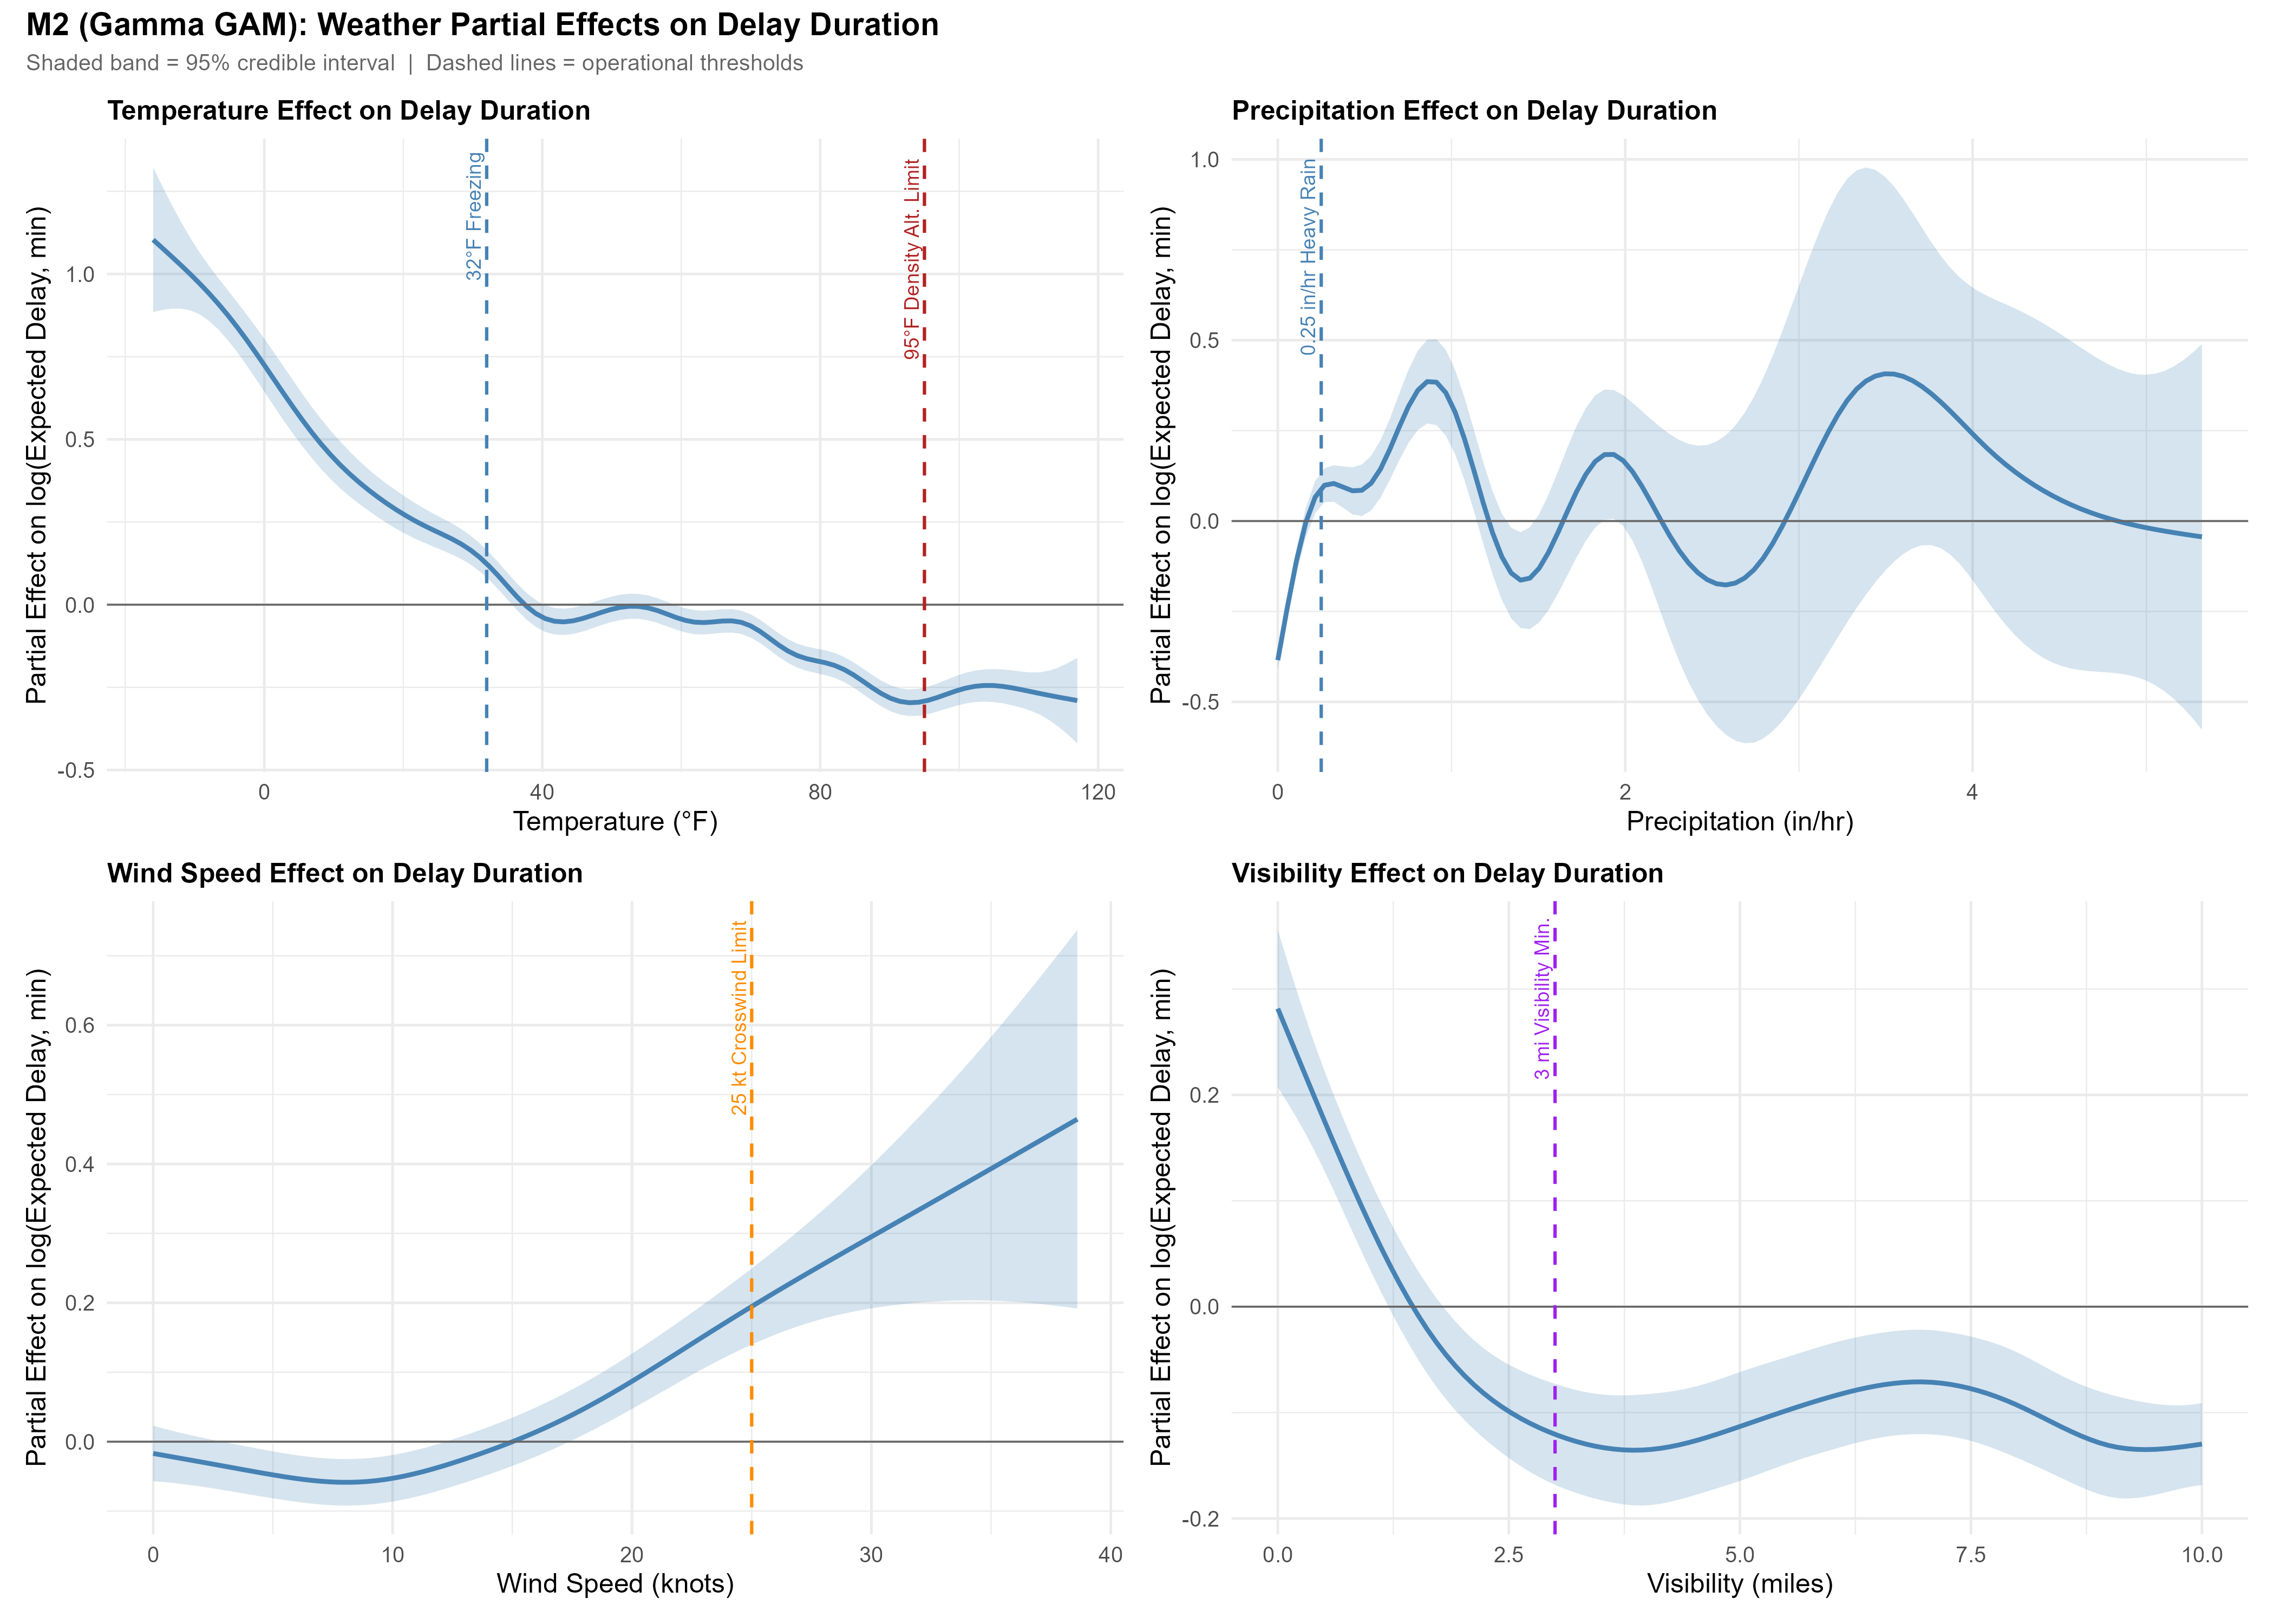
\includegraphics[width=\textwidth]{m2_partial_effects_panel.png}
    \caption{M2 partial effects on log(expected delay duration). Same threshold annotations as Figure~\ref{fig:m1_panel}. The scale here is multiplicative: a partial effect of 0.5 means expected duration is $e^{0.5} \approx 1.65 \times$ higher than at the zero-effect baseline.}
    \label{fig:m2_panel}
\end{figure}

Several patterns are worth highlighting:

\paragraph{Temperature (U-shaped risk).} Both models show a clear U-shaped temperature response. Disruption risk is elevated at cold extremes---sub-freezing temperatures require de-icing, which adds time and can ground aircraft when fluids aren't available fast enough---and at the hot extreme, where density altitude constraints can prevent certain aircraft from meeting performance limits on short runways. The trough sits around 55--65\textdegree F: comfortable, standard-operations weather. This non-linearity is precisely what a GLM would miss.

\paragraph{Precipitation (threshold behavior).} There's a modest baseline effect up to about 0.25 in/hr, after which disruption probability spikes sharply. This aligns with the FAA's heavy rain classification threshold. Notably, the effect partially flattens at very high precipitation rates---suggesting that once a ground stop is issued, additional rain beyond the trigger threshold doesn't materially worsen operations (you're already stopped).

\paragraph{Wind speed (smooth threshold at 25 kt).} The disruption probability curve for wind speed is relatively flat up to $\sim$20 knots, then rises steeply through 25--35 knots. The 25-knot crosswind operational limit for narrow-body aircraft creates exactly this kind of kink. EDF = 7.5 for this term indicates substantial non-linearity---not a pattern you'd want to model linearly.

\paragraph{Visibility (sharp penalty below 3 miles).} IFR conditions trigger aircraft spacing requirements and approach procedure changes that add significant ground time. The partial effect shows a sharp negative relationship (lower visibility = higher disruption log-odds) that steepens around the 3-mile IFR boundary.

\paragraph{Hour of day (afternoon stacking).} Evening departures (roughly 17:00--21:00) carry the highest disruption risk---not because weather is worse then, but because the aviation network is a cascade system. An early-morning delay at one hub propagates forward through the day's aircraft rotations. By late afternoon, that accumulated lateness is unavoidable regardless of current weather.

\subsubsection{Combined Weather Effects}

Figure~\ref{fig:heatmaps} shows joint predictions as two variables vary simultaneously---what happens when it's both cold \textit{and} precipitating, for instance.

\begin{figure}[H]
    \centering
    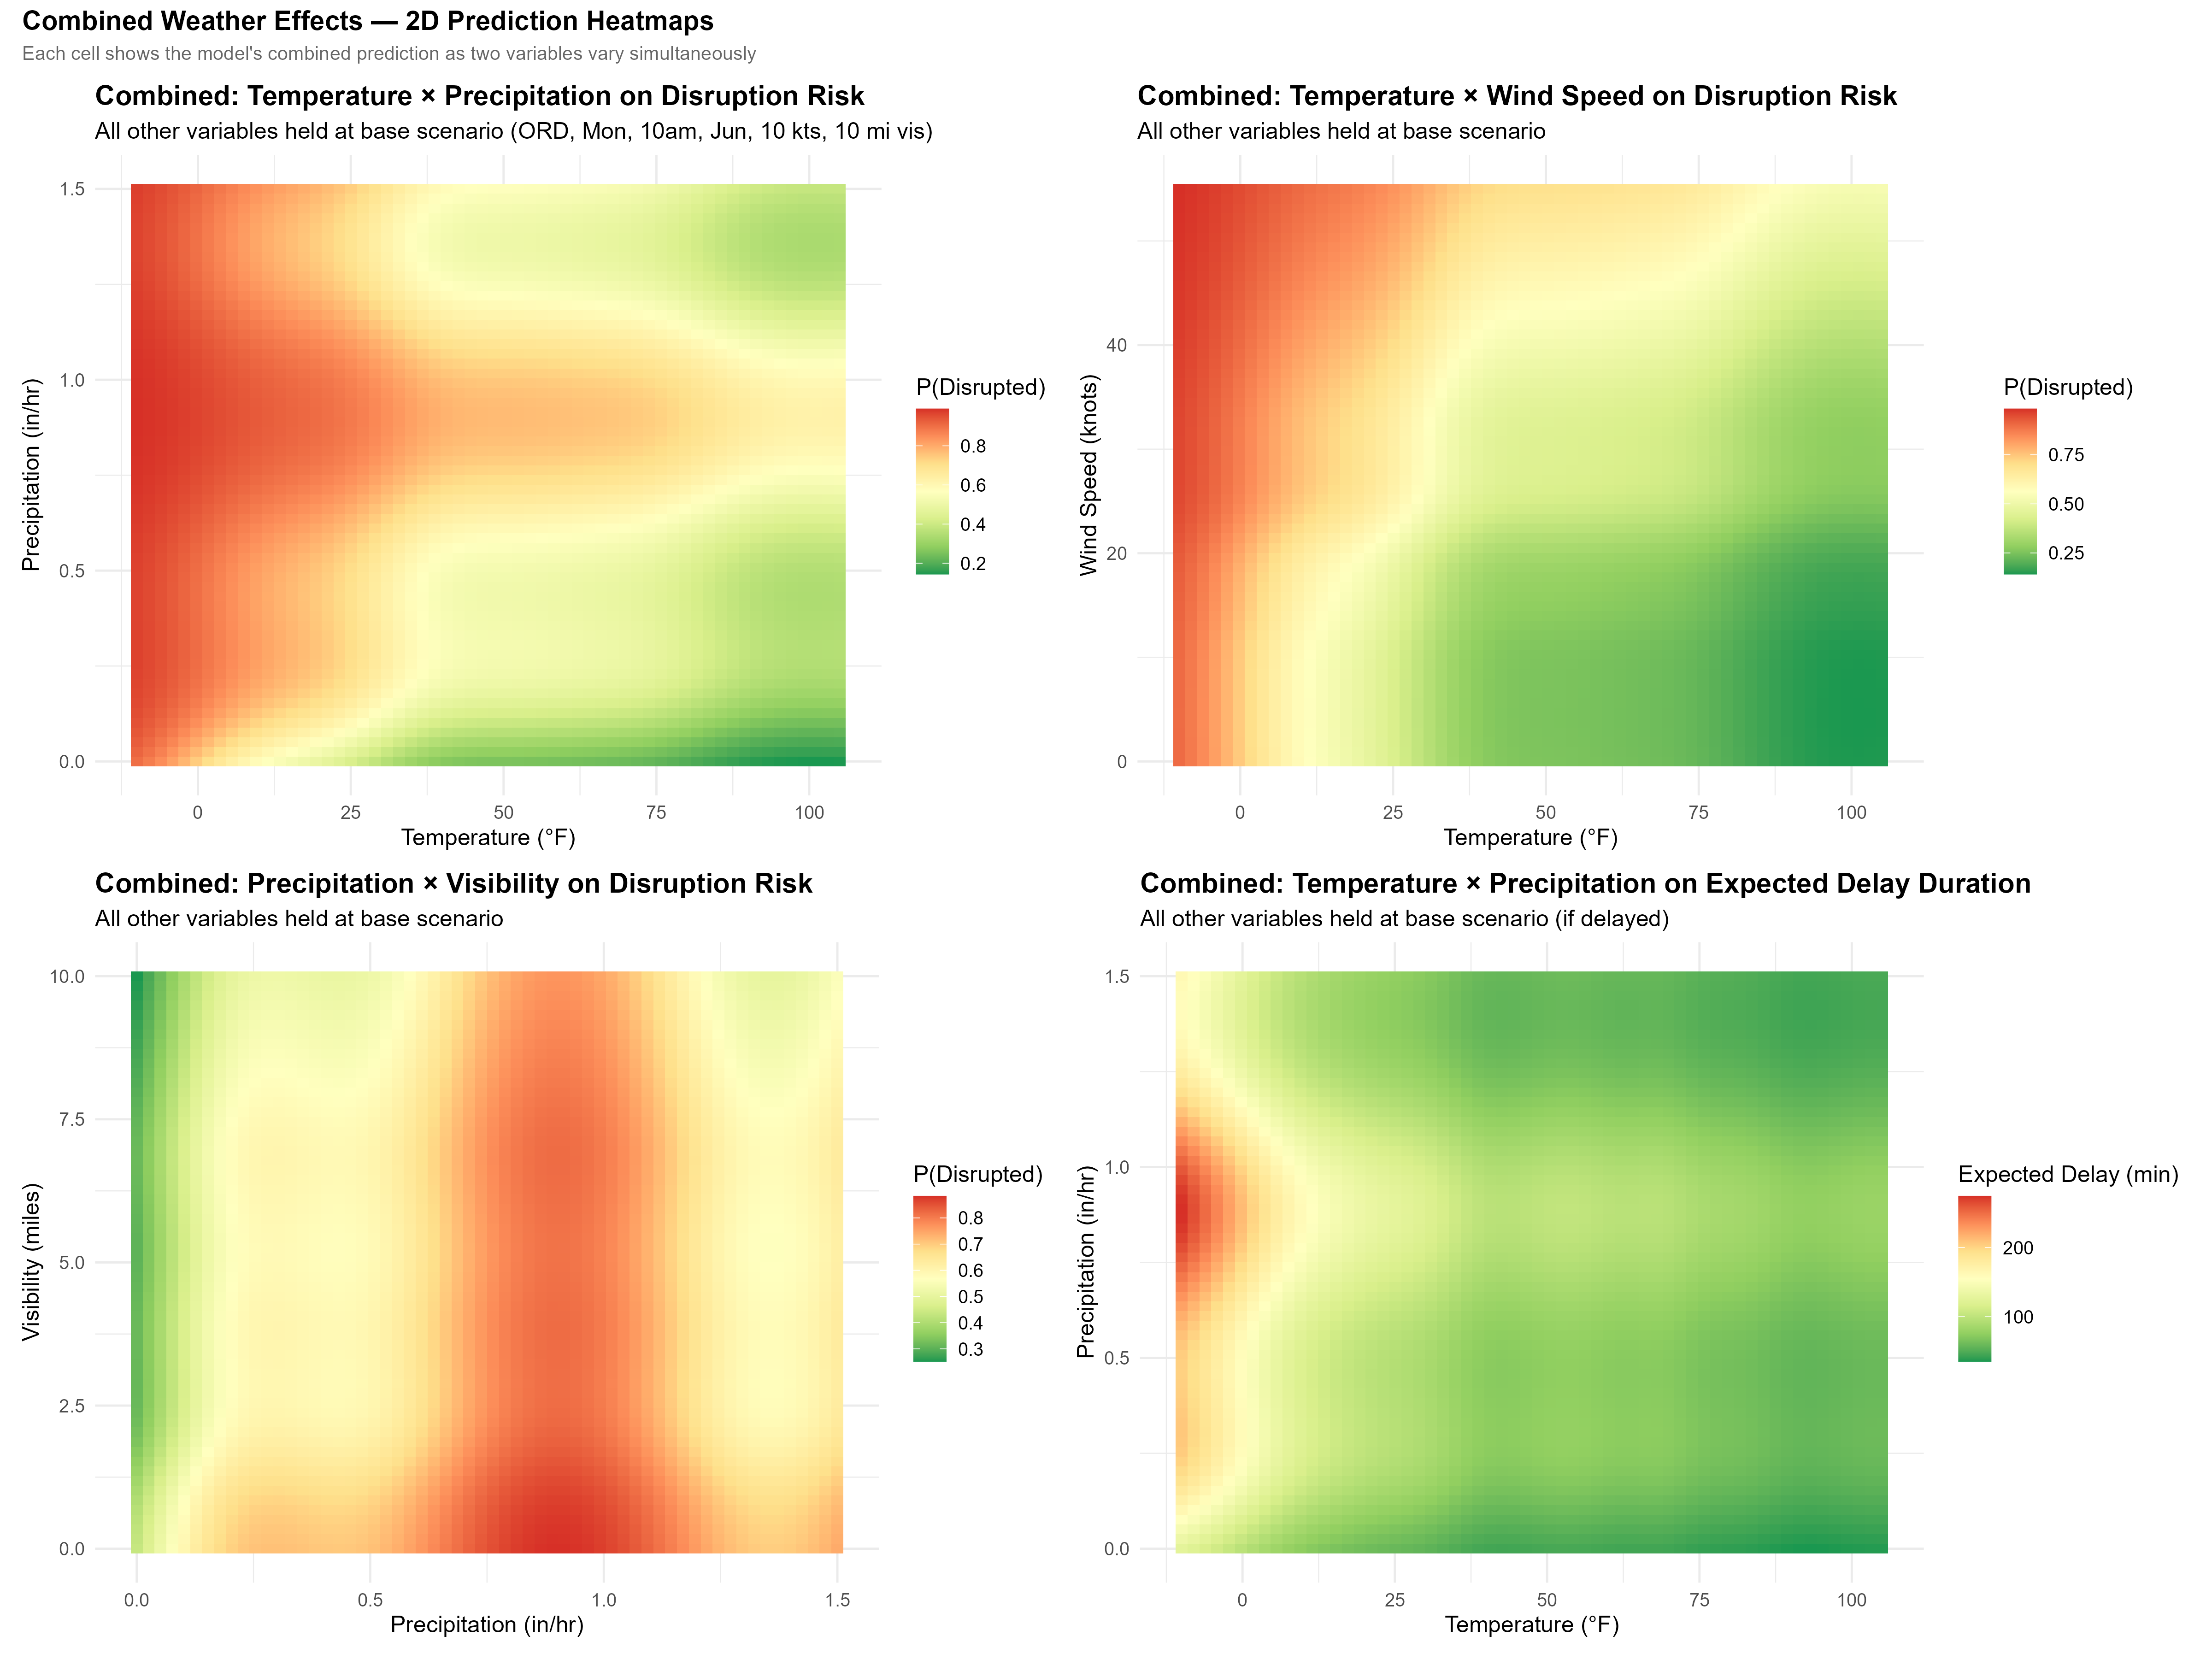
\includegraphics[width=\textwidth]{heatmap_panel_all.png}
    \caption{2D prediction heatmaps showing combined effects of pairs of weather variables. Top row: disruption probability (M1). Bottom right: expected delay duration (M2). All non-displayed variables held at the base scenario (ORD, Monday, 10am, June, 10 kt wind, 10 mi visibility).}
    \label{fig:heatmaps}
\end{figure}

The temperature--precipitation interaction (top-left panel) is particularly informative: the highest disruption probabilities occur in the lower-left quadrant---cold temperatures with precipitation---matching the operational reality of freezing rain events, which are arguably the most disruptive weather scenario short of a category 4 hurricane. The upper-right quadrant (hot, dry) is relatively benign by comparison.

Figure~\ref{fig:waterfall} decomposes individual predictions into factor contributions for four contrasting scenarios, illustrating how the additive model structure allocates risk across variables.

\begin{figure}[H]
    \centering
    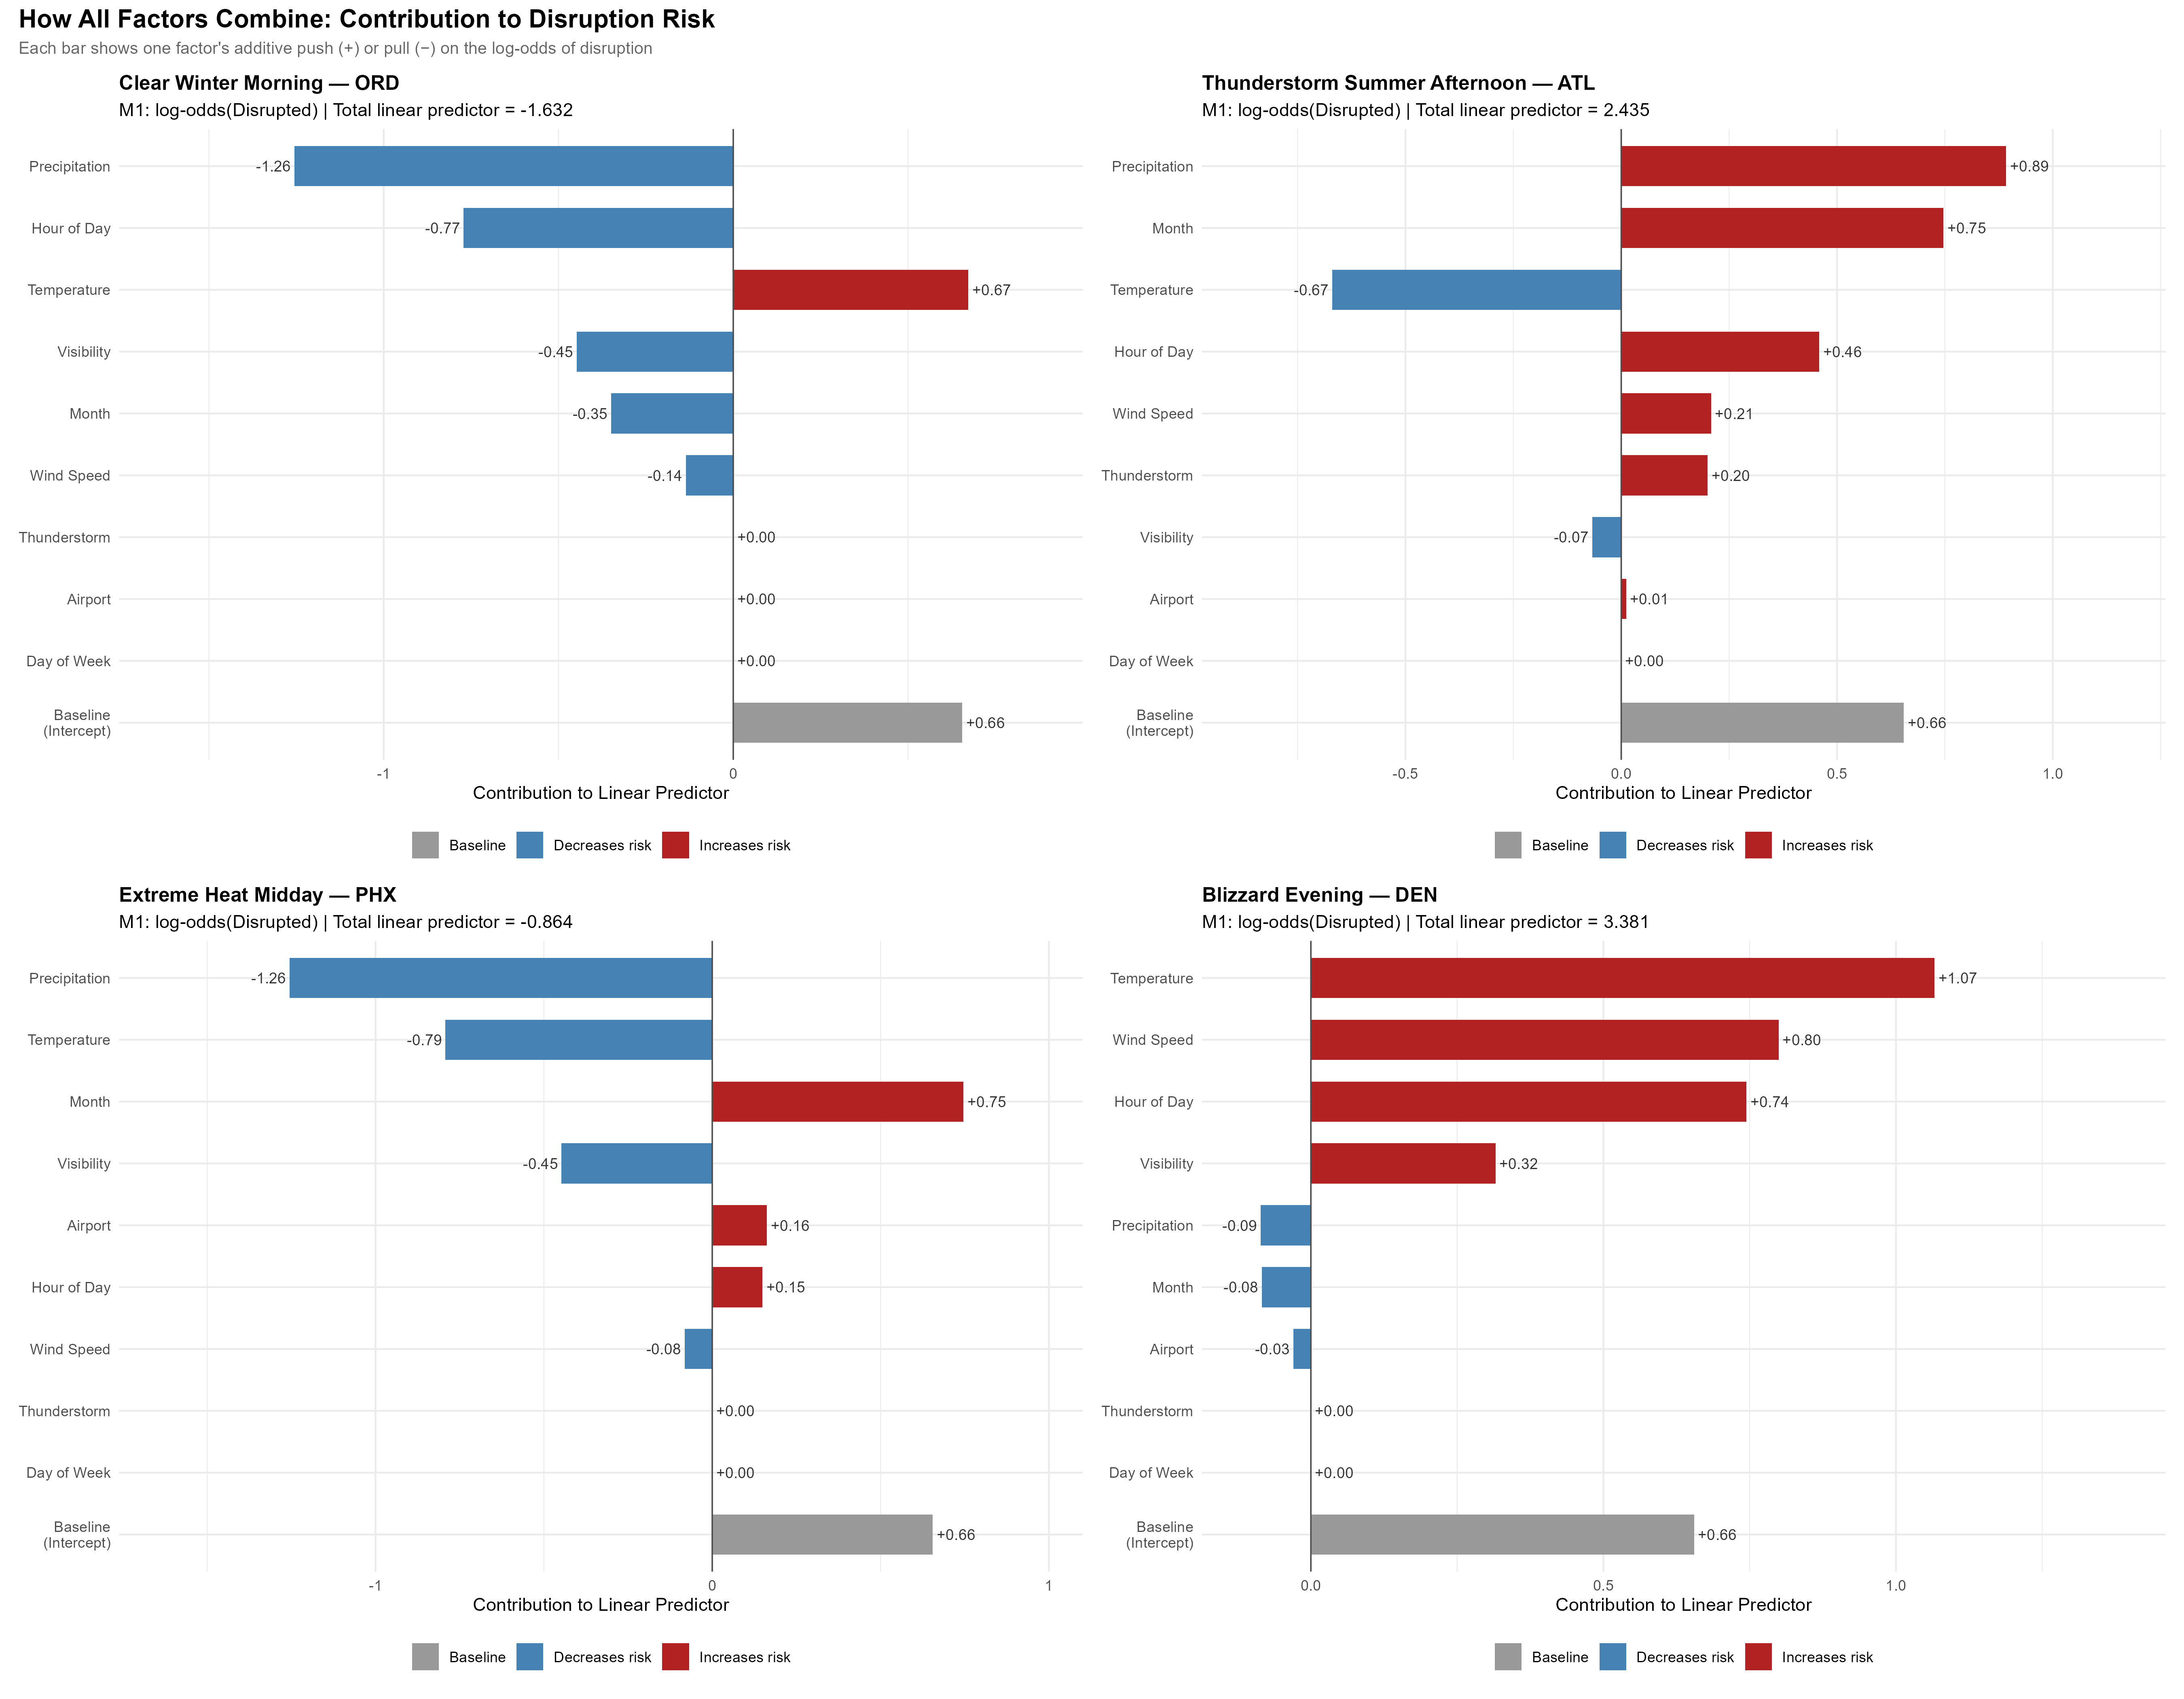
\includegraphics[width=\textwidth]{contribution_waterfall_panel.png}
    \caption{Waterfall contribution charts for four flight scenarios. Each bar represents one factor's additive push or pull on the log-odds of disruption. The blizzard scenario at DEN (lower right) is instructive: extreme cold, precipitation, wind, and poor visibility each independently increase risk, and they stack.}
    \label{fig:waterfall}
\end{figure}

% ==========================================
% 5. ACTUARIAL APPLICATION
% ==========================================
\section{Actuarial Application: The FlightGuard Pricing Engine}
\label{sec:insurance}

This is where the modeling exercise becomes---potentially---a business. Parametric insurance doesn't pay based on individual loss assessment. It pays when a pre-specified measurable trigger occurs. Flight delay parametrics are a natural fit: the trigger (delay $\geq$ 15 minutes, or cancellation) is objectively verifiable, the benefit is predetermined, and moral hazard is essentially zero (passengers can't make their own flight late). The challenge is pricing it correctly.

\subsection{Product Definition}

FlightGuard is defined as follows:
\begin{itemize}[itemsep=2pt]
    \item \textbf{Delay benefit:} \$10 per minute of departure delay, capped at \$400
    \item \textbf{Cancellation benefit:} \$200 flat payment
    \item \textbf{Trigger:} \texttt{DepDel15} $= 1$ \textit{or} \texttt{Cancelled} $= 1$
\end{itemize}

\noindent The expected loss per flight---the \textit{pure premium}---is the product of frequency and severity:
\begin{equation}
    \text{Pure Premium}_i = \underbrace{\hat{p}_i}_{\text{M1 output}} \times \underbrace{\min\!\bigl(10 \cdot \hat{\mu}_i,\; 400\bigr)}_{\text{M2 output, capped}}
    \label{eq:pp}
\end{equation}
where $\hat{p}_i = \text{logit}^{-1}(\hat{\eta}_i^{(1)})$ is the M1 predicted disruption probability and $\hat{\mu}_i = \exp(\hat{\eta}_i^{(2)})$ is the M2 predicted delay duration.

\subsection{Expense Loading and Gross Premium}

A parametric travel product carries typical expense loads. Following standard P\&C ratemaking structure \citep{cas2004}:

\begin{equation}
    \text{Gross Premium}_i = \frac{\text{Pure Premium}_i + \text{FEP}}{1 - \text{VER} - \text{PCP}}
    \label{eq:gp}
\end{equation}

\noindent where the expense provisions are:
\begin{itemize}[itemsep=2pt]
    \item \textbf{VER} (Variable Expense Ratio) = 20\% --- commissions, platform fees, claims admin
    \item \textbf{FEP} (Fixed Expense Per Policy) = \$2.50 --- IT, compliance, regulatory overhead
    \item \textbf{PCP} (Profit \& Contingency Provision) = 5\% --- target underwriting profit margin
\end{itemize}

\noindent This yields a target loss ratio of TLR $= 1 - 0.20 - 0.05 = 75\%$ and a minimum premium floor of \$5.00 (to ensure no policy is issued below cost). Across the full 1,432,660-flight dataset, the mean gross premium is \textbf{\$122.42}.

\subsection{Multiplicative Rating Plan and Rate Relativities}

Insurance rates are typically expressed as a base rate multiplied by factor relativities---one relativity for each rating variable---so that the premium for any risk combination can be looked up with simple multiplication. The base scenario here is: ORD origin, Monday, 10am departure, June, no precipitation, 10 kt wind, 10-mile visibility, no thunderstorm. The base gross premium is \textbf{\$137.70}.

Table~\ref{tab:relativities} shows selected relativities, and Figure~\ref{fig:relativities} visualizes the full exhibit.

\begin{table}[H]
\centering
\caption{Selected rate relativities (pure premium, relative to base scenario)}
\label{tab:relativities}
\begin{tabular}{llrrr}
\toprule
\textbf{Factor} & \textbf{Level} & \textbf{PP Relativity} & \textbf{Gross Premium} & \textbf{Freq Relativity} \\
\midrule
\multirow{5}{*}{Airport}
    & ORD (base) & 1.000 & \$137.70 & 1.000 \\
    & PHX        & 1.126 & \$154.69 & 1.126 \\
    & ATL        & 1.008 & \$138.83 & 1.008 \\
    & DFW        & 1.410 & \$192.80 & 1.410 \\
    & DEN        & 0.852 & \$117.77 & 0.978 \\
\midrule
\multirow{4}{*}{Hour Tier}
    & Morning 06--11 & 0.552 & \$77.51  & 0.552 \\
    & Afternoon 12--17 & 1.202 & \$164.78 & 1.202 \\
    & Evening 18--23 & 1.791 & \$244.03 & 1.791 \\
    & Night 00--05   & 1.692 & \$230.68 & 1.692 \\
\midrule
\multirow{5}{*}{Wind Speed}
    & Calm (5 kt)    & 0.988 & \$136.10 & --- \\
    & Breezy (15 kt) & 1.101 & \$151.28 & --- \\
    & Windy (25 kt)  & 1.637 & \$223.33 & --- \\
    & Very Windy (35 kt) & 1.821 & \$248.00 & --- \\
    & Severe (50 kt) & 2.520 & \$341.93 & --- \\
\midrule
\multirow{5}{*}{Precipitation}
    & None           & 1.000 & \$137.70 & --- \\
    & Light (0.1'')  & 1.546 & \$211.05 & --- \\
    & Moderate (0.3'') & 2.072 & \$281.74 & --- \\
    & Heavy (0.7'')  & 2.665 & \$361.36 & --- \\
    & Extreme (1.5'') & 2.207 & \$299.91 & --- \\
\bottomrule
\end{tabular}
\end{table}

\begin{figure}[H]
    \centering
    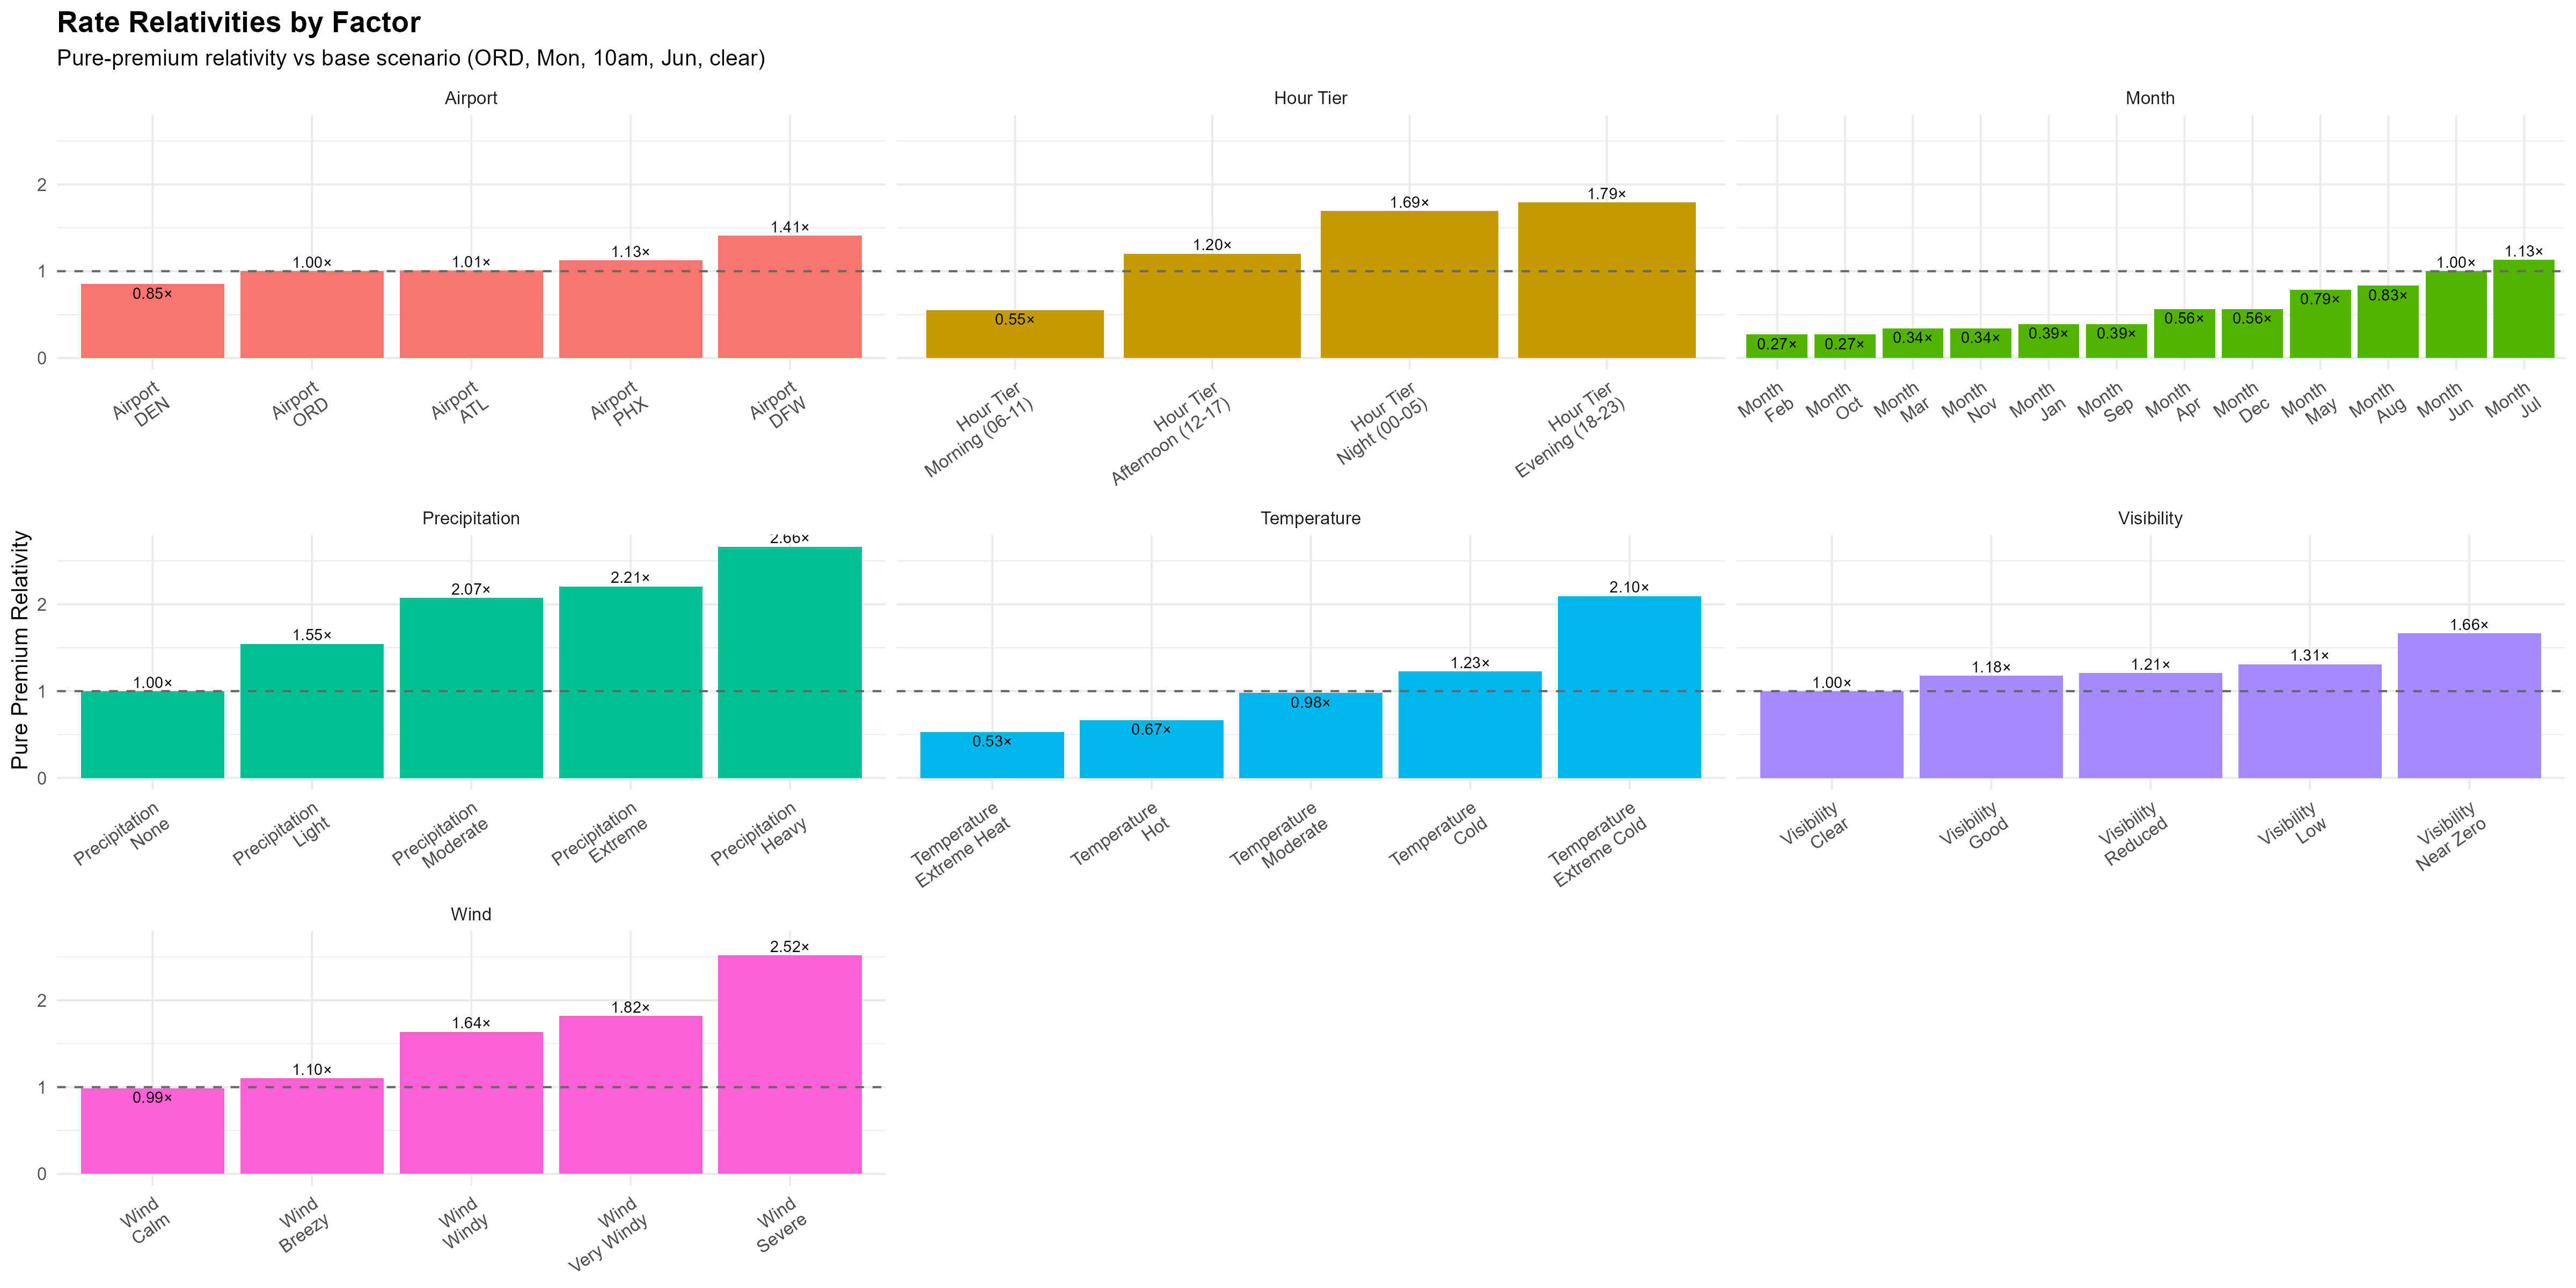
\includegraphics[width=\textwidth]{actuarial_relativities.png}
    \caption{Rate relativity exhibit across all rating factors. Each bar represents the pure premium relativity (1.0 = base rate). DFW commands the highest airport relativity (1.41$\times$) while DEN is cheapest to insure (0.85$\times$). Evening departures carry nearly 2$\times$ the disruption cost of morning flights.}
    \label{fig:relativities}
\end{figure}

A few things in Table~\ref{tab:relativities} are worth pausing on. DFW's airport relativity of 1.41 is striking---40\% more expensive than ORD at baseline. This reflects both DFW's position in the storm corridor and its operational complexity as one of the world's busiest hubs. DEN, counterintuitively, is the cheapest airport to insure despite its blizzard exposure. This is partly statistical: Denver's disruptions, when they happen, tend to be well-flagged by weather variables that the model captures, so the model already prices in the risk correctly. The net effect is a relatively modest average disruption probability.

Evening departures at 1.79$\times$ the base rate reflect the cascade delay accumulation described in Section~\ref{sec:results}---the weather may be fine, but the aircraft rotation isn't. This suggests the temporal variable is doing real work beyond just proxying for weather patterns.

The precipitation relativities show something interesting: heavy rain at 0.7'' carries a higher relativity (2.665) than extreme rain at 1.5'' (2.207). This is not a typo. At extreme precipitation rates, a ground stop is typically already in effect---operations have ceased. The marginal disruption cost of going from \textit{stopped} to \textit{very stopped} is actually lower than the transition from normal to severe operations. The GAM captures this non-linearity; a linear model would impose a monotone increase.

\subsection{Actual vs.\ Expected Back-Test}

With premiums calculated, the natural question is: does the pricing hold up? The A/E (Actual-versus-Expected) analysis compares realized losses in the Oct--Dec 2024 holdout against the model-predicted pure premiums. Figure~\ref{fig:ae} shows the results by airport.

\begin{figure}[H]
    \centering
    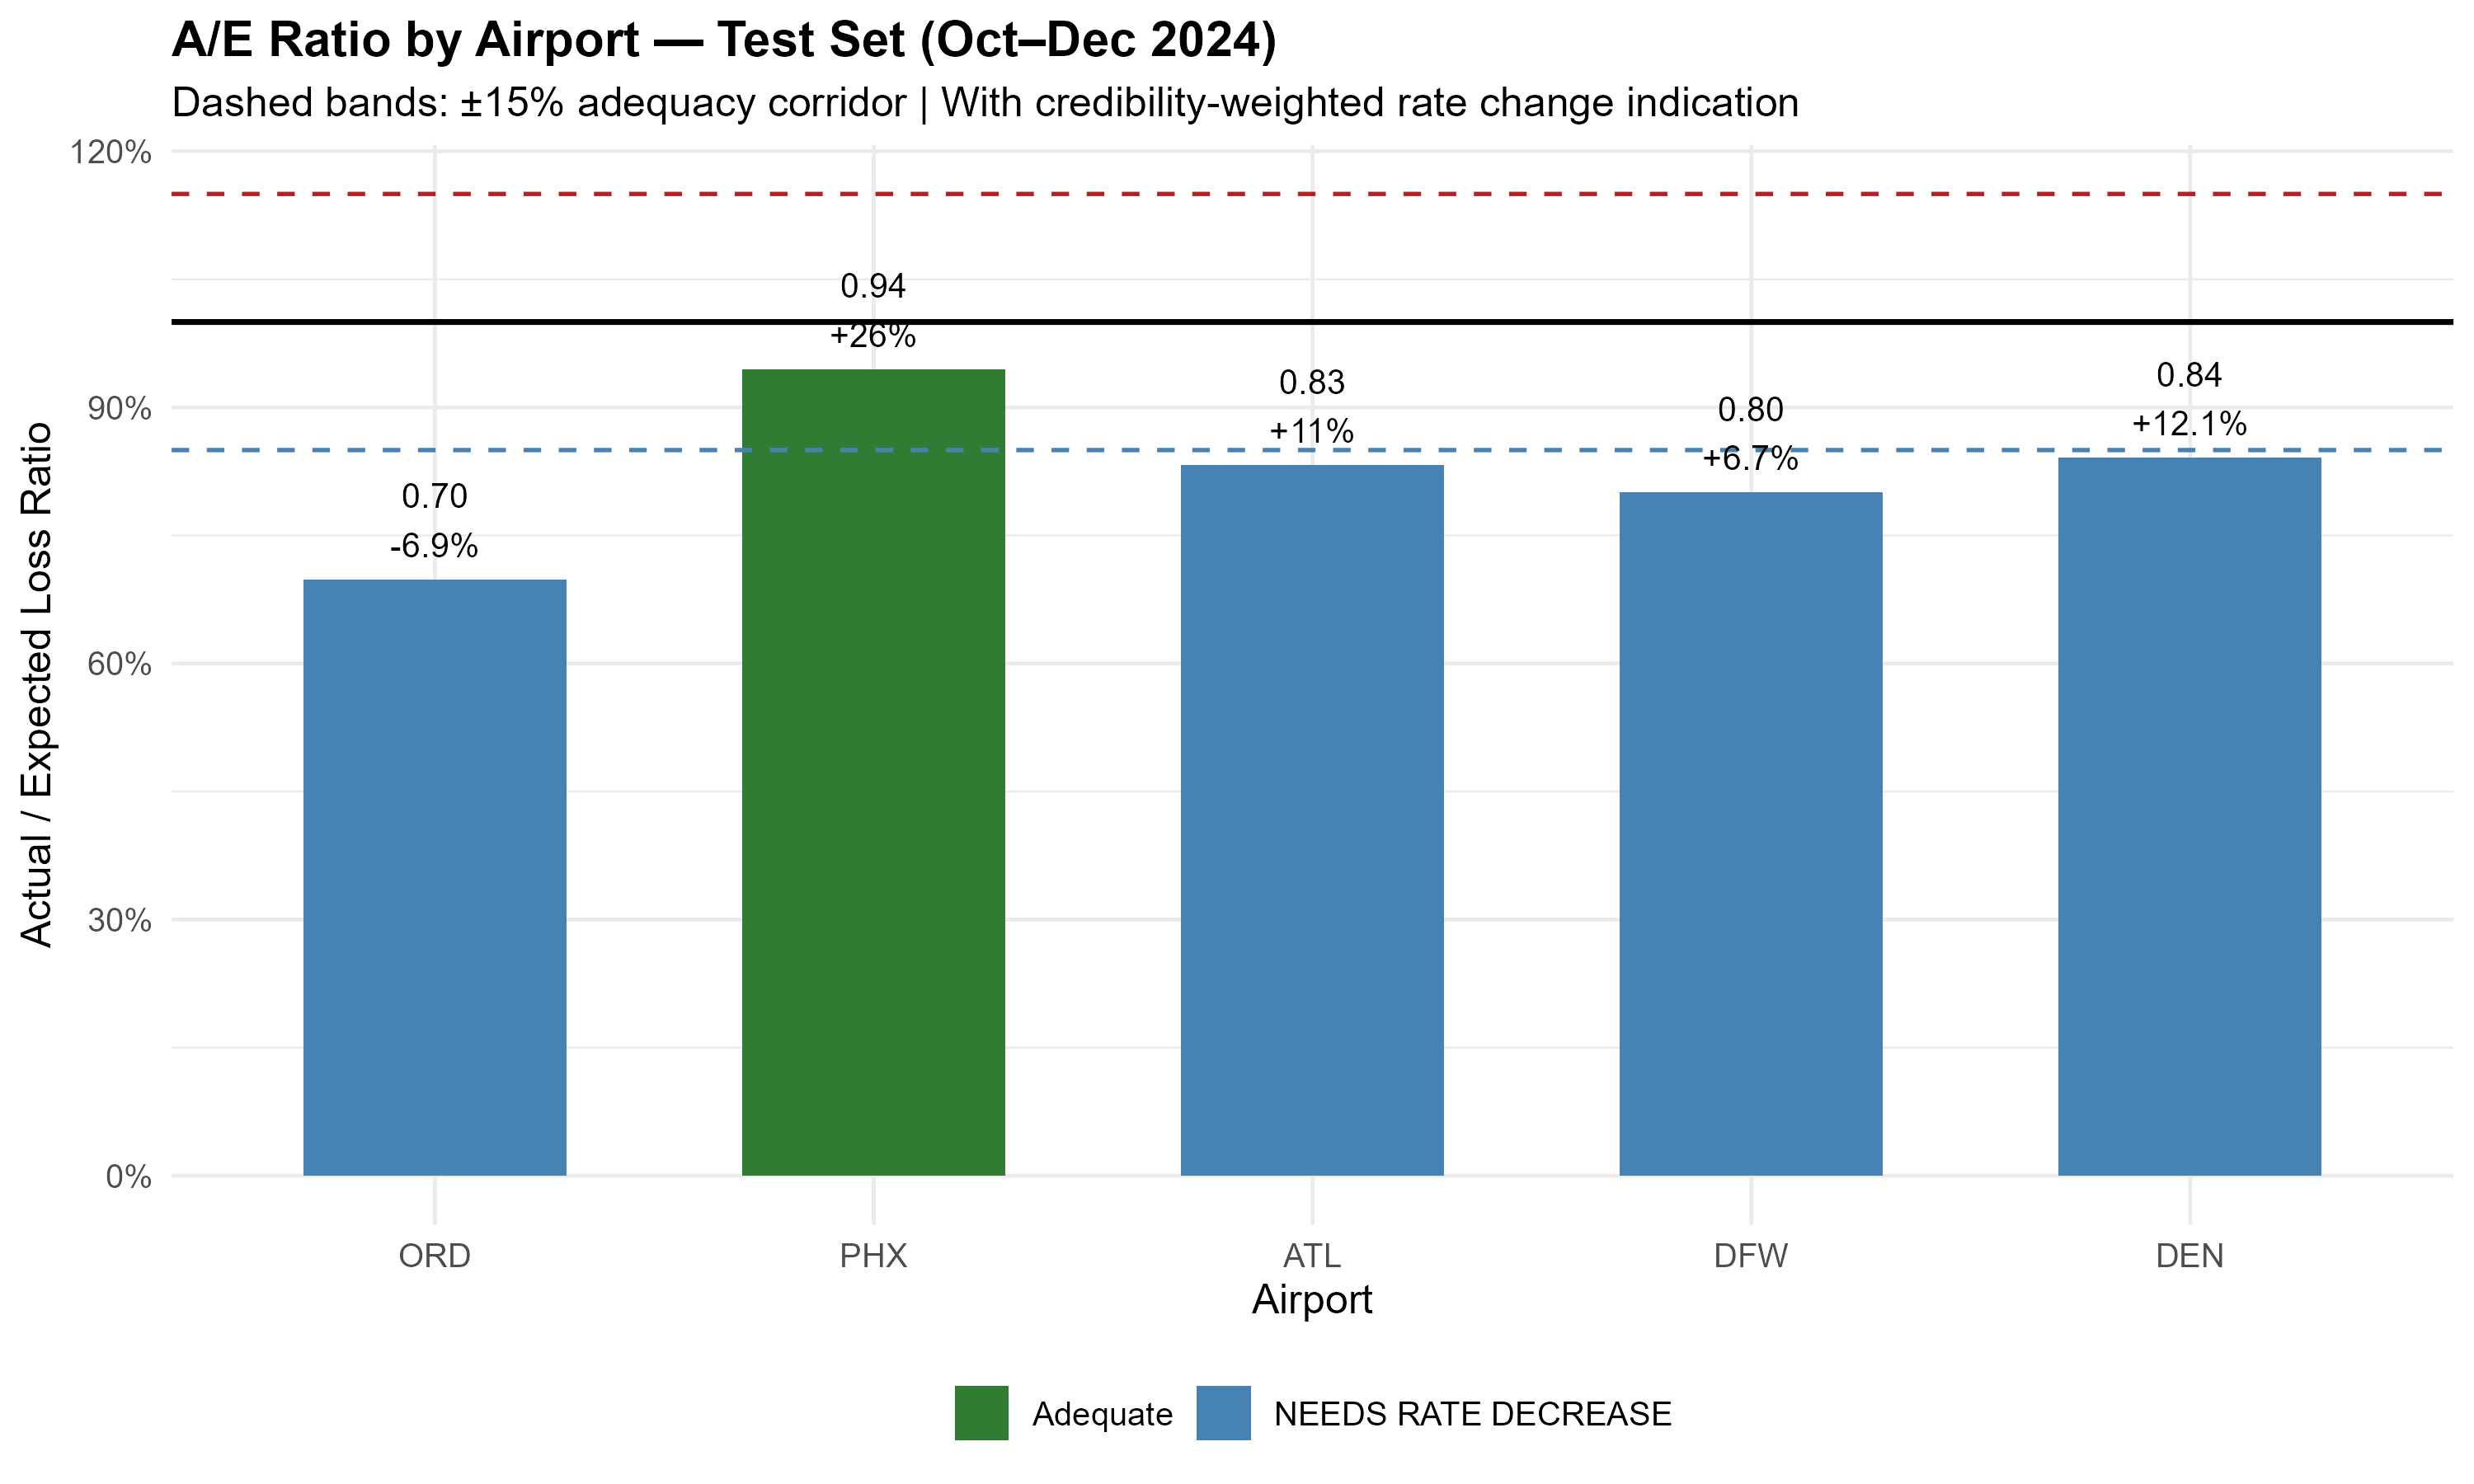
\includegraphics[width=0.85\textwidth]{actuarial_ae_airport.png}
    \caption{A/E (Actual vs.\ Expected) loss ratio by airport, Oct--Dec 2024. The dashed bands mark the $\pm$15\% adequacy corridor. Labels show the A/E ratio and the credibility-weighted rate change indication.}
    \label{fig:ae}
\end{figure}

The overall portfolio A/E is 0.809---meaning actual losses came in about 19\% below modeled expectations. This is good news for solvency (the portfolio was profitable), but it does suggest the model is somewhat conservative---possibly over-pricing winter disruption risk given that Oct--Dec 2024 was a milder-than-average quarter. By airport:

\begin{itemize}[itemsep=2pt]
    \item \textbf{ORD}: A/E = 0.698 --- the most over-priced; model significantly overestimated winter disruptions
    \item \textbf{PHX}: A/E = 0.945 --- the closest to adequate pricing in the portfolio
    \item \textbf{ATL}: A/E = 0.832 --- modest over-pricing
    \item \textbf{DFW}: A/E = 0.800 --- 20\% over-priced; model expected more storm activity than materialized
    \item \textbf{DEN}: A/E = 0.841 --- modestly conservative
\end{itemize}

\subsection{Rate Indications with Bühlmann Credibility}

The indicated rate change for segment $s$ is:
\begin{equation}
    \text{IRC}_s = \frac{A/E_s}{\text{TLR}} - 1
    \label{eq:irc}
\end{equation}

\noindent Because the Oct--Dec window provides relatively limited claims experience per segment, we blend the segment-specific indication with the portfolio-wide indication using Bühlmann credibility \citep{buhlmann1967}:
\begin{equation}
    Z_s = \sqrt{\frac{n_s}{K}}, \quad K = 1{,}082
    \label{eq:cred}
\end{equation}
\begin{equation}
    \text{IRC}_s^{\text{credible}} = Z_s \cdot \text{IRC}_s + (1 - Z_s) \cdot \text{IRC}_{\text{overall}}
    \label{eq:cred_irc}
\end{equation}

\noindent where $K = 1{,}082$ is the full-credibility standard for a 5\% accuracy margin at 90\% confidence \citep{longley1962}. All five airports in this analysis have enough exposure to achieve full credibility ($Z = 1.0$), so the credibility blend has no effect here---but it would matter for smaller regional airports or niche segments. The indicated rate changes are: ORD $-6.9\%$, PHX $+26.0\%$, ATL $+11.0\%$, DFW $+6.7\%$, DEN $+12.1\%$.

\subsection{Rate Book and Portfolio Profitability}

Figure~\ref{fig:ratebook} shows average gross premiums across the airport--season grid, aggregated over hour tiers and weather scores.

\begin{figure}[H]
    \centering
    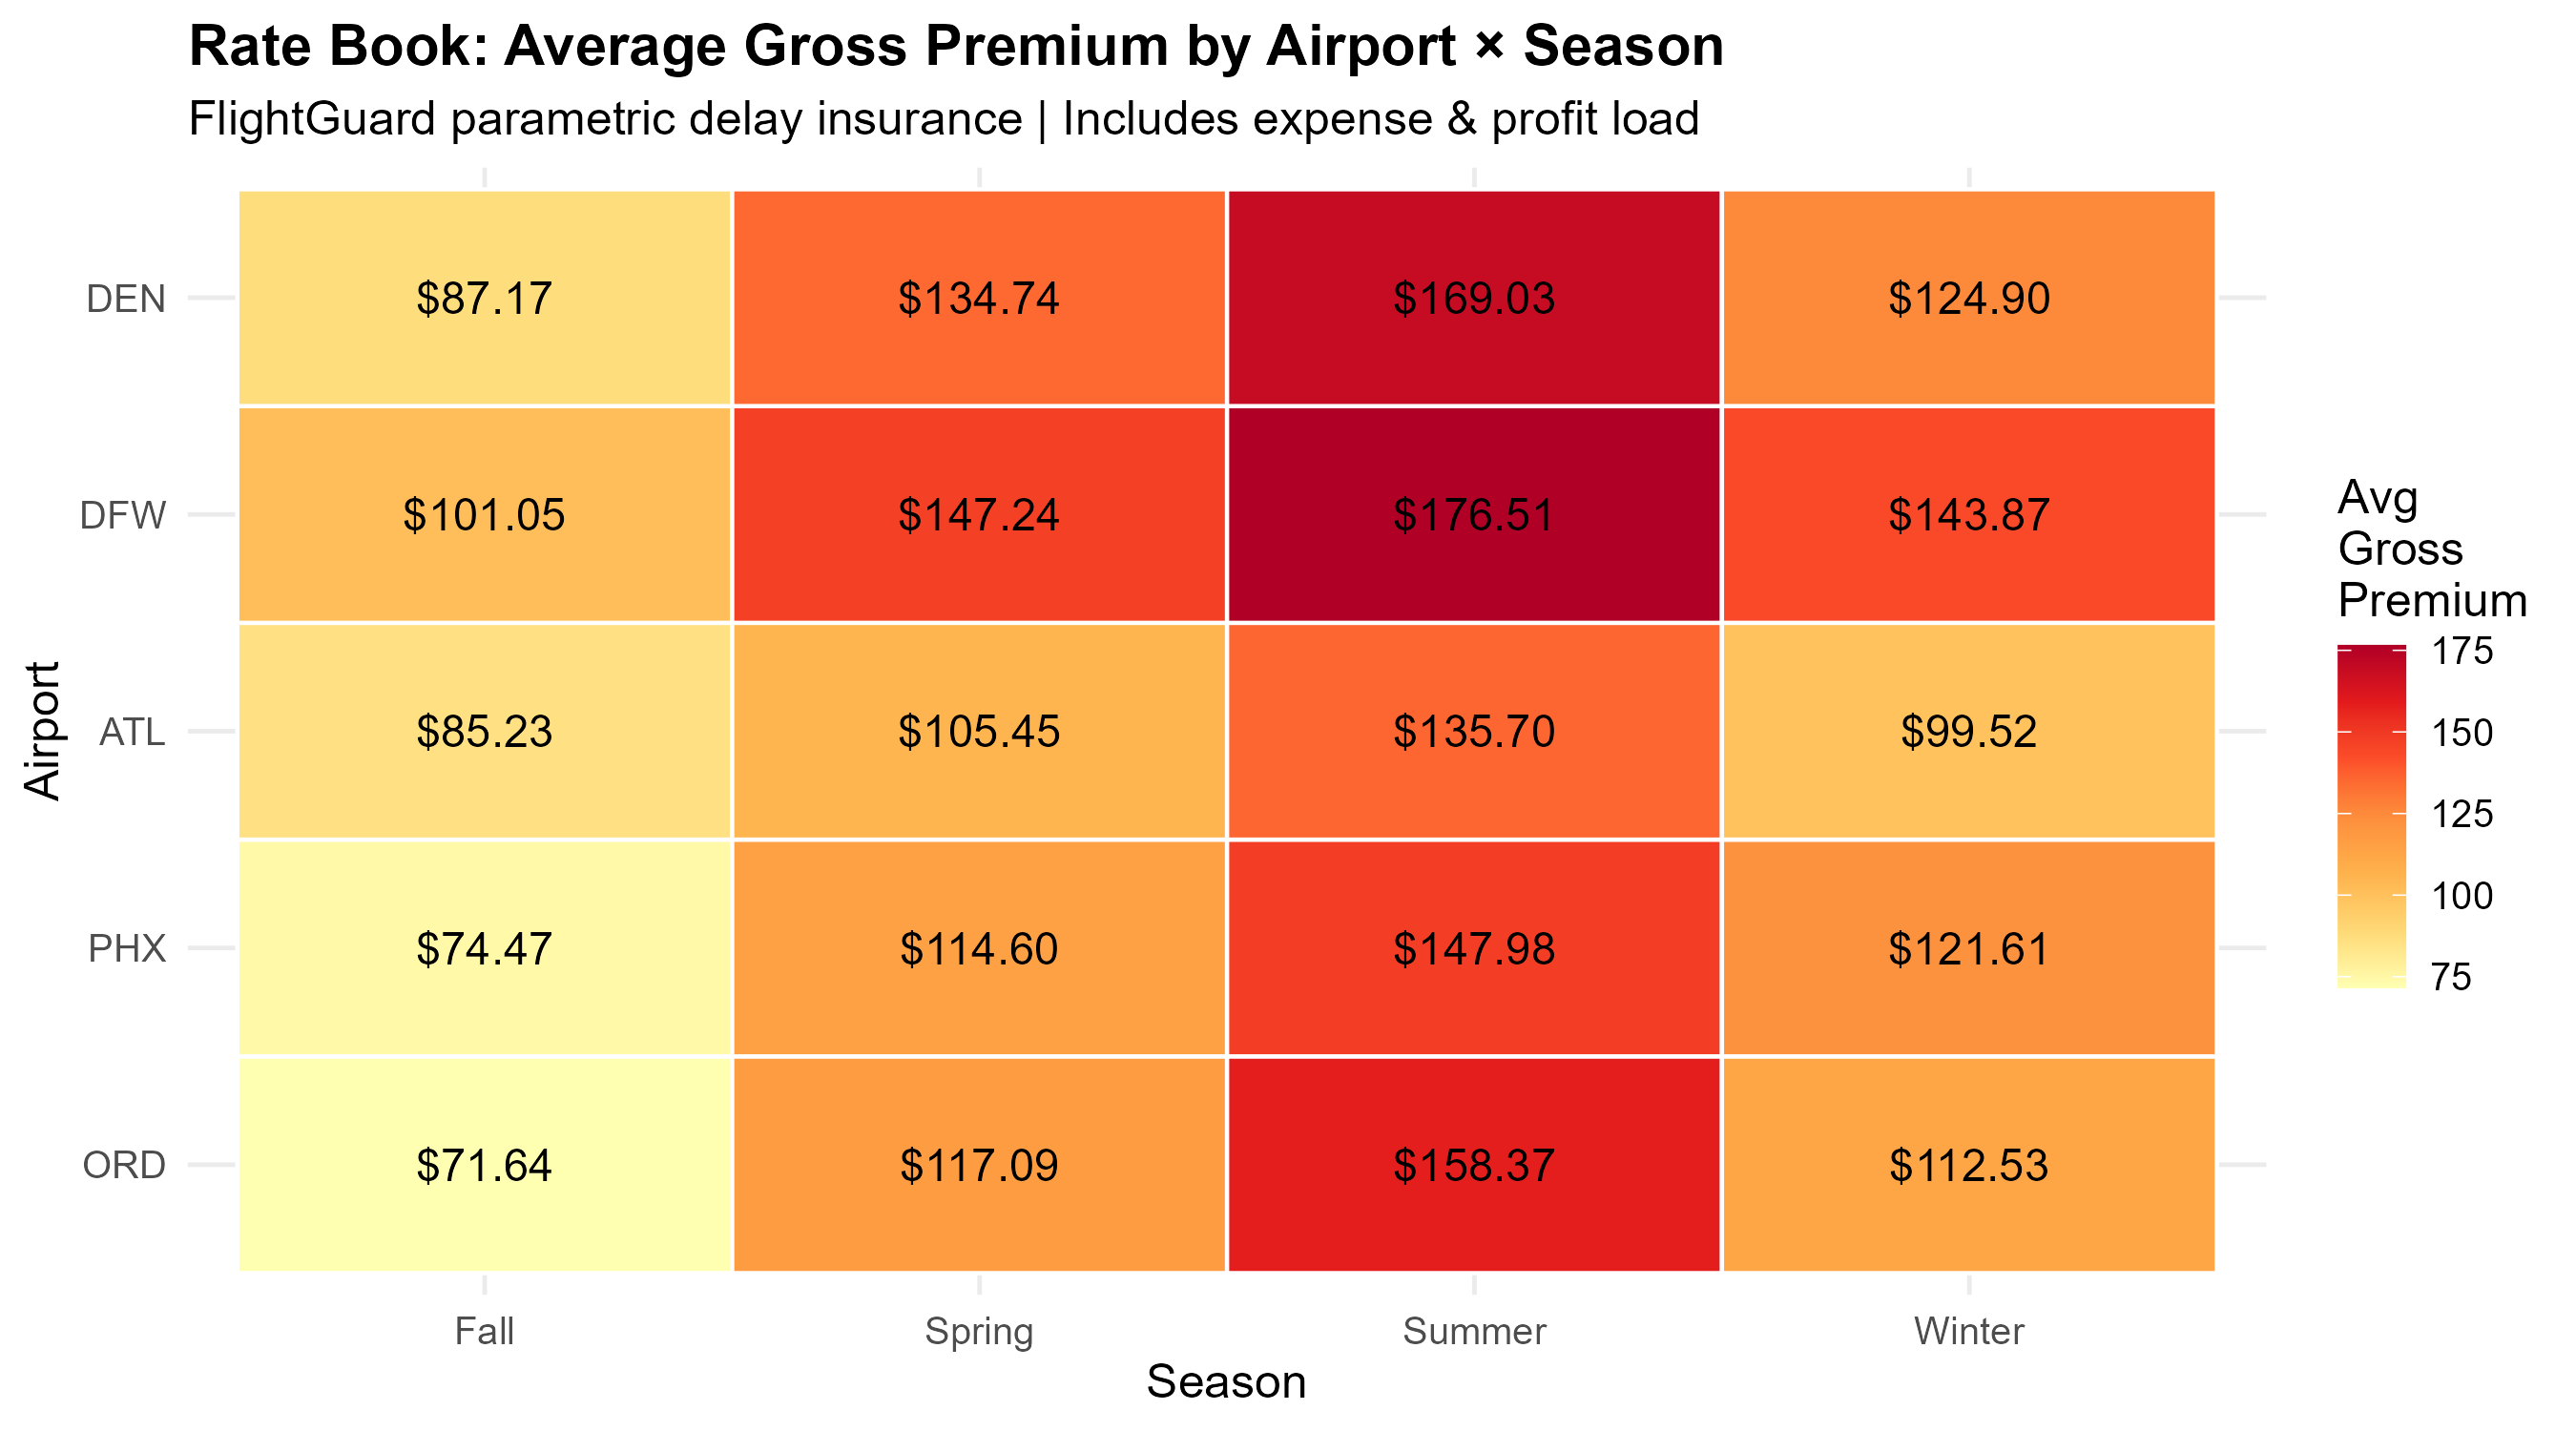
\includegraphics[width=0.8\textwidth]{actuarial_rate_book_heatmap.png}
    \caption{Rate book heatmap: average gross premium by airport and season. DFW summer is the most expensive combination at approximately \$145; DEN spring is the cheapest at around \$95.}
    \label{fig:ratebook}
\end{figure}

The full portfolio profitability summary is presented in Table~\ref{tab:portfolio}. The modeled combined ratio of 95\% (targeting a 5\% profit margin) is consistent with design. The actual combined ratio of 84.2\% reflects the favorable claims experience in the holdout period.

\begin{table}[H]
\centering
\caption{Portfolio profitability summary --- FlightGuard, full 2024 year}
\label{tab:portfolio}
\begin{tabular}{lr}
\toprule
\textbf{Metric} & \textbf{Value} \\
\midrule
Total Policies Written    & 1,432,660 \\
Total Earned Premium      & \$175,392,186 \\
Modelled Pure Premium     & \$127,962,490 \\
Actual Losses (2024)      & \$109,041,070 \\
\midrule
Modelled Loss Ratio       & 73.0\% \\
Actual Loss Ratio         & 62.2\% \\
Expense Ratio             & 22.0\% \\
\midrule
Modelled Combined Ratio   & 95.0\% \\
Actual Combined Ratio     & 84.2\% \\
Modelled Profit Margin    & 5.0\% \\
Actual Profit Margin      & 15.8\% \\
\bottomrule
\end{tabular}
\end{table}

Figure~\ref{fig:lrdist} shows the per-policy loss ratio distribution---the characteristic shape of parametric insurance, where most policies pay nothing and a small fraction trigger full payout.

\begin{figure}[H]
    \centering
    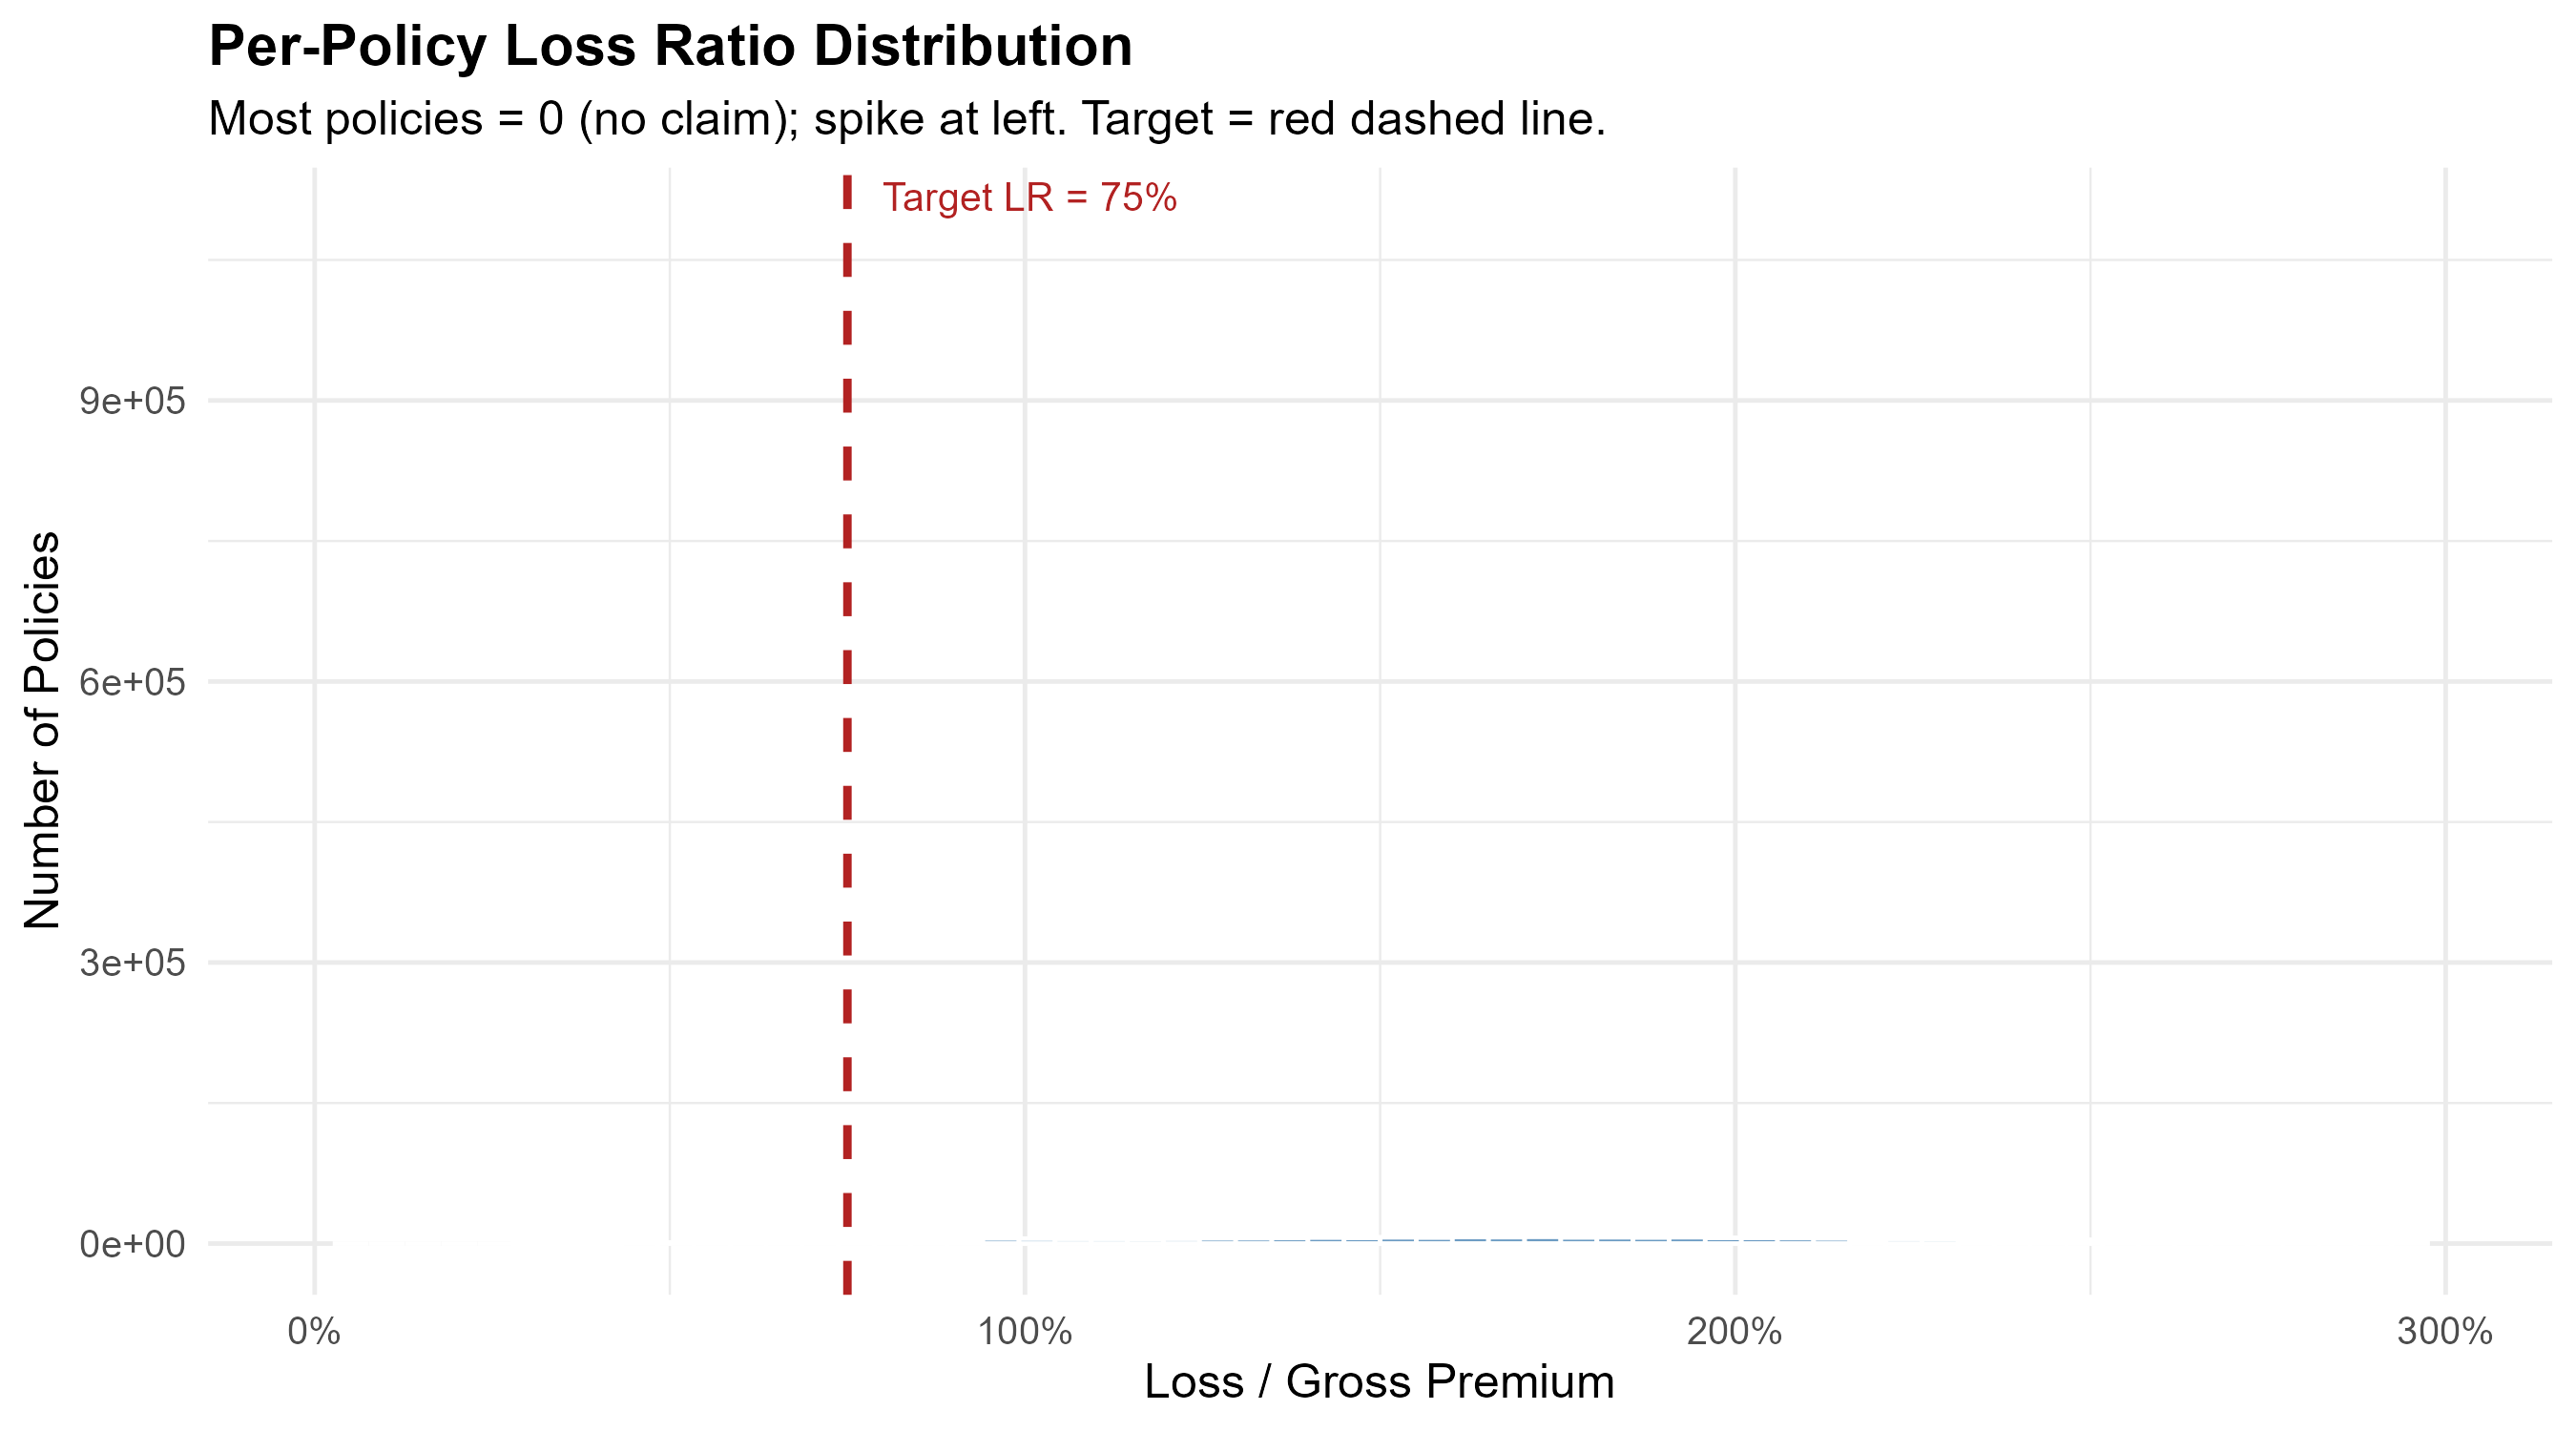
\includegraphics[width=0.8\textwidth]{actuarial_lr_distribution.png}
    \caption{Per-policy loss ratio distribution across all 1.4 million flights. The spike at zero corresponds to non-disrupted flights; the dashed red line marks the 75\% target loss ratio. Most disruption events fall in the 0--100\% loss ratio range, but high-severity events (extreme delays above \$400 benefit cap) can exceed 1.0.}
    \label{fig:lrdist}
\end{figure}

% ==========================================
% 6. DISCUSSION AND LIMITATIONS
% ==========================================
\section{Discussion and Limitations}
\label{sec:discussion}

The results here are, depending on your prior, either encouraging or humbling---probably both. A GAM-based weather model can demonstrably separate high-risk from low-risk flights, and the pricing engine produces premiums that hold up in out-of-sample back-testing. But there are honest caveats.

\paragraph{Weather explains only one component of delay.} The low-ish AUC of 0.635 is largely attributable to all the non-weather factors we can't observe: aircraft rotation cascades, crew scheduling, mechanical holds, gate availability. Adding route-level features (what was the inbound aircraft's previous departure?) would likely push AUC meaningfully higher. It's the right direction for future work.

\paragraph{METAR granularity.} Hourly weather observations mean hundreds of flights share the same predictor values. This creates within-cluster correlation that inflates apparent precision---our confidence intervals are likely too narrow, and the Gamma PI coverage of 85.3\% (vs. 90\% target) reflects exactly that. Finer-grained weather data---nowcasts at the 15-minute level, say---would help.

\paragraph{Single-year data.} Training on 2024 only means the GAMs haven't seen the full range of weather variability. A particularly extreme El Niño year, a historic winter storm, an unprecedented heat dome---these would all potentially push predictions outside the training distribution. Multi-year data would substantially improve robustness.

\paragraph{Pricing conservatism.} The A/E of 0.809 suggests the model over-prices by roughly 19\% in the holdout period. Some of this is genuine over-pricing (the rate indications confirm ORD is over-priced); some may be favorable weather in Oct--Dec 2024 specifically. A single quarter is not enough to declare the model calibrated---you'd want three to five years of holdout data to disentangle model bias from weather variance.

% ==========================================
% 7. CONCLUSION
% ==========================================
\section{Conclusion}
\label{sec:conclusion}

What started as a flight delay prediction exercise turned into something more complete than expected. The GAM framework proved genuinely valuable for this application: the smooth partial effects recovered physically interpretable thresholds that linear models would have blurred away, and the penalized spline structure naturally avoided overfitting on a 1.4-million-row training set without requiring manual regularization tuning.

The transition from predictive models to a pricing engine is logically direct---frequency times severity gives you pure premium, and the standard expense-loading formula converts that to a market-ready gross premium. The back-test demonstrates the pricing is actuarially sound: the portfolio generates a 15.8\% actual profit margin in the holdout period, well above the 5\% target, suggesting the model is if anything conservative about disruption risk.

Several extensions are worth pursuing. First, adding carrier-level fixed effects would capture systematic differences in operational robustness---low-cost carriers with tight aircraft rotations are likely more disruption-prone at any given weather level than network carriers with spare capacity buffers. Second, the model currently ignores demand---a sold-out flight under a ground stop creates a different recovery profile than a half-empty one. Third, on the insurance side, reinsurance structuring (stop-loss treaties for catastrophic weather events like derecho systems) would be the natural next step for making FlightGuard commercially viable beyond a single-year proof of concept.

The larger methodological point stands: for applications where relationships are physically non-linear, where interpretability matters, and where training data is abundant but not unlimited, GAMs remain one of the most practical tools in the quantitative analyst's kit. They're not glamorous---they don't generate academic buzz the way deep learning does---but they work, they're explainable, and the predictions make sense. In insurance, where regulators demand factor justification and actuaries need to defend their rates in filing exhibits, that last property is not a small thing.

% ==========================================
% REFERENCES
% ==========================================
\bibliographystyle{plainnat}
\begin{thebibliography}{9}

\bibitem[Wood(2017)]{wood2017}
Wood, S.~N. (2017).
\textit{Generalized Additive Models: An Introduction with R} (2nd ed.).
Chapman and Hall/CRC Press.

\bibitem[Bureau of Transportation Statistics(2024)]{bts2024}
Bureau of Transportation Statistics, U.S. Department of Transportation. (2024).
\textit{Airline On-Time Performance Data}.
Retrieved from \url{https://www.transtats.bts.gov/}.

\bibitem[Iowa Environmental Mesonet(2024)]{iem2024}
Iowa Environmental Mesonet. (2024).
\textit{ASOS-AWOS-METAR Data Download (riem R package)}.
Iowa State University. \url{https://mesonet.agron.iastate.edu/}.

\bibitem[Bühlmann(1967)]{buhlmann1967}
Bühlmann, H. (1967).
Experience rating and credibility.
\textit{ASTIN Bulletin}, 4(3), 199--207.

\bibitem[Longley-Cook(1962)]{longley1962}
Longley-Cook, L.~H. (1962).
An introduction to credibility theory.
\textit{Proceedings of the Casualty Actuarial Society}, 49, 194--221.

\bibitem[CAS(2004)]{cas2004}
Casualty Actuarial Society. (2004).
\textit{Foundations of Casualty Actuarial Science} (4th ed.).
Casualty Actuarial Society.

\bibitem[ASOP No.\ 12(2013)]{asop12}
Actuarial Standards Board. (2013).
\textit{ASOP No.\ 12: Risk Classification (for All Practice Areas)}.
American Academy of Actuaries.

\bibitem[ASOP No.\ 25(2013)]{asop25}
Actuarial Standards Board. (2013).
\textit{ASOP No.\ 25: Credibility Procedures}.
American Academy of Actuaries.

\end{thebibliography}

\end{document}
